% main.tex
\documentclass[11pt,a4paper,oneside]{book}

% ---------- Packages ----------
\usepackage[utf8]{inputenc}
\usepackage[T1]{fontenc}
\usepackage[english]{babel}
\usepackage{lmodern}
\usepackage{microtype}
\usepackage{graphicx}
\usepackage{hyperref}
\usepackage{geometry}
\usepackage{enumitem}
\usepackage{booktabs}
\usepackage{xcolor}
\usepackage{listings}
\usepackage{fancyhdr}

\geometry{margin=2.5cm}
\graphicspath{{Imagenes/}}

% Friendly callout box
\newcommand{\encourage}[1]{%
  \vspace{0.5em}
  \noindent\colorbox{gray!10}{\parbox{\dimexpr\linewidth-2\fboxsep\relax}{\textit{#1}}}
  \vspace{0.5em}
}

% ---------- Code blocks ----------
\lstset{
  basicstyle=\ttfamily\small,
  columns=fullflexible,
  frame=single,
  breaklines=true,
  postbreak=\mbox{\textcolor{gray}{$\hookrightarrow$}\space},
}
\hypersetup{hypertexnames=false}
% ---------- Header / Footer ----------
\pagestyle{fancy}
\fancyhf{}
\lhead{Digital Sovereignty Manual}
\rhead{\nouppercase{\leftmark}}
\cfoot{\thepage}
\setlength{\headheight}{14pt}

% Make chapter-opening pages use the same header/footer (book uses 'plain' there)
\fancypagestyle{plain}{
  \fancyhf{}
  \lhead{Digital Sovereignty Manual}
  \rhead{\nouppercase{\leftmark}}
  \cfoot{\thepage}
  \setlength{\headheight}{14pt}
}

% Improve chapter marks (avoid "CHAPTER X" clutter in headers)
\renewcommand{\chaptermark}[1]{\markboth{#1}{}}

% ---------- Metadata ----------
\title{Digital Sovereignty in Practice\\ \large Self-hosted services with Docker: Photos, Music, Local AI, and Private Drive}
\author{Mattia Coccolo}
\date{\today}

% ---------- Custom title page (editorial: floating title + vertically centered image) ----------
\makeatletter
\renewcommand{\maketitle}{%
  \begin{titlepage}
    \thispagestyle{empty}
    \centering

    % --- Top: floating title block ---
    \vspace*{1.3cm}
    {\Huge\bfseries Digital Sovereignty\par}
    \vspace{0.15cm}
    {\Huge\bfseries in Practice\par}
    \vspace{0.45cm}
    {\large Self-hosted services with Docker: Photos, Music, Local AI, and Private Drive\par}

    % --- Middle: vertically centered image ---
    \vfill
    
\includegraphics[width=0.62\textwidth]{Imagenes/serivdor_rey}
    \vfill

    % --- Bottom: author + date (quiet) ---
    {\large Mattia Coccolo\par}
    \vspace{0.15cm}
    {\small \today\par}

    \vspace*{1.0cm}
  \end{titlepage}
}
\makeatother

% --- Watermark / corner logo on odd pages only (GLOBAL, compatible) ---
\usepackage{eso-pic}
\usepackage{transparent}

\newcommand{\OddCornerMark}{%
  \AddToShipoutPictureFG{%
    \ifodd\value{page}
      \AtPageUpperLeft{%
        \raisebox{-30.2cm}{% baja desde arriba
          \hspace*{18.8cm}% desplaza hacia la derecha (ajusta)
          \transparent{1}%
          
\includegraphics[width=2.2cm]{serivdor_rey_agua}%
        }%
      }%
    \fi
  }%
}
\begin{document}

\frontmatter
\maketitle

\cleardoublepage
\chapter*{License}
\addcontentsline{toc}{chapter}{License}

\noindent\textbf{Text and code:}\\
Creative Commons Attribution--NonCommercial--ShareAlike 4.0 International (CC BY-NC-SA 4.0)

\vspace{0.8em}

\noindent\textbf{Illustrations:}\\
Creative Commons Attribution--NonCommercial--NoDerivatives 4.0 International (CC BY-NC-ND 4.0)

\vspace{1.0em}

\noindent\textbf{Links:}\\
\url{https://creativecommons.org/licenses/by-nc-sa/4.0/}\\
\url{https://creativecommons.org/licenses/by-nc-nd/4.0/}

\vspace{1.0em}

\noindent\textbf{Attribution:}\\
\copyright\ \the\year\ Mattia Coccolo.

\vspace{0.6em}

\noindent\textbf{Permissions:}\\
For permissions beyond these licenses (e.g., commercial use or adaptations of illustrations), please contact the author.

\tableofcontents

% chapters/00_prologue.tex
\chapter*{Prologue}
\addcontentsline{toc}{chapter}{Prologue}

\begin{center}
  \vspace{0.6cm}
  
\includegraphics[width=0.38\textwidth]{serivdor_perplejo}
  \vspace{0.8cm}
\end{center}


This manual is a practical, step-by-step guide to building your own small digital ecosystem: a private photo library, a music server, local AI tools, and a personal cloud drive---all running on your own machine, under your control, with Docker as the backbone.

The motivation is simple: most of our digital lives live somewhere else. Photos, documents, messages, research notes, calendars, passwords, and even our work routines are increasingly mediated by services we do not operate. This can be convenient, but convenience often comes with hidden costs: lock-in, recurring subscriptions, opaque data practices, and a quiet dependence on decisions made far from our needs and values.

The goal here is not to reject the internet or to chase an unrealistic ideal of ``total independence''. The goal is to show that a meaningful level of \emph{digital sovereignty} is achievable with accessible tools: electricity, internet, a computer, and a bit of patience. You can keep your core data at home (or at your institution), expose only what you choose, and still enjoy modern usability.

This manual is written for people who want to:
\begin{itemize}[leftmargin=*]
  \item understand what they run and where their data lives,
  \item reduce dependence on external platforms without sacrificing daily convenience,
  \item create a modular setup that can evolve over time,
  \item document the process so it can be reproduced by colleagues, friends, or students.
\end{itemize}

\section*{A note on scope}
\addcontentsline{toc}{section}{A note on scope}

We focus on a pragmatic stack:
\begin{itemize}[leftmargin=*]
  \item \textbf{Docker + Linux} as the foundation,
  \item \textbf{PhotoPrism} for photos,
  \item \textbf{Navidrome} for music,
  \item \textbf{Local AI} (Ollama + a web UI) for private, on-device workflows,
  \item \textbf{A private drive} (e.g., Seafile) for syncing and organizing files.
\end{itemize}

We will also briefly discuss operational concerns: storage layout, backups, updates, and basic security choices. Whenever something depends on a specific environment (home server vs. university server, VPN vs. public exposure), we explicitly say so.

\section*{How to use this manual}
\addcontentsline{toc}{section}{How to use this manual}

Each chapter follows a predictable pattern:
\begin{itemize}[leftmargin=*]
  \item \textbf{Goal}: what you will have at the end,
  \item \textbf{Prerequisites}: what you need beforehand,
  \item \textbf{Steps}: the actions to perform,
  \item \textbf{Verification}: how to confirm it works,
  \item \textbf{Troubleshooting}: the common failure modes and fixes.
\end{itemize}

If you already have a Docker host running, you can skip directly to the service chapters (PhotoPrism, Navidrome, Local AI, and the Private Drive). If you only want one service, you can treat chapters as independent modules.

\section*{Philosophy: small, modular, reproducible}
\addcontentsline{toc}{section}{Philosophy: small, modular, reproducible}

This manual aims for:
\begin{itemize}[leftmargin=*]
  \item \textbf{Small steps}: avoid ``big bang'' setups. Make one thing work, then add the next.
  \item \textbf{Modularity}: each service lives in its own container(s), with clear volumes and ports.
  \item \textbf{Reproducibility}: all configuration should be portable via compose files and a documented folder structure.
\end{itemize}

Done well, the result feels less like ``running servers'' and more like owning your own digital workspace.


\mainmatter
\OddCornerMark
% chapters/01_intro_digital_sovereignty.tex
\chapter{Digital Sovereignty: what it is, and why it matters}


\begin{center}
  \vspace{0.6cm}
  
\includegraphics[width=0.38\textwidth]{serivdor_rey}
  \vspace{0.8cm}
\end{center}


\section{A working definition}
Digital sovereignty is the ability to \emph{choose} how your digital life works:
\begin{itemize}[leftmargin=*]
  \item where your data is stored,
  \item who can access it (and under what conditions),
  \item how services evolve over time,
  \item what happens if a provider changes rules, prices, or policies.
\end{itemize}

It is not a binary state. It is a spectrum. The question is not ``sovereign or not'', but \emph{how much control you want} and \emph{where it is worth the effort}.

\section{Why it matters (even if you are not ``technical'')}
There are four recurring reasons people move toward more sovereignty:

\subsection{Control and resilience}
Platforms change. Features disappear. Prices rise. Accounts get locked. Terms of service shift. A self-hosted core makes your workflow more resilient: if one component fails, you still own your data and can migrate.

\subsection{Privacy and confidentiality}
For researchers, professionals, and anyone handling personal archives, privacy is not a luxury. Local-first tools reduce the need to upload sensitive content to third parties by default.

\subsection{Cost transparency}
Many cloud services start free and become expensive at scale (storage, team accounts, add-ons). With self-hosting, costs are mostly upfront (hardware, disks) and predictable (electricity, backups). That trade-off often becomes favorable once you have non-trivial archives (photos, videos, datasets).

\subsection{Freedom from lock-in}
When your data and workflows depend on proprietary formats or closed ecosystems, switching becomes painful. Using standard tools and keeping raw files under your control makes migration a choice, not a crisis.

\section{Threat model: what are we protecting against?}
Before installing anything, define what you care about. A minimal threat model answers:
\begin{itemize}[leftmargin=*]
  \item \textbf{Loss}: disk failure, accidental deletion, ransomware.
  \item \textbf{Exposure}: services reachable from the public internet without safeguards.
  \item \textbf{Lock-in}: dependence on one provider or one app.
  \item \textbf{Downtime}: updates breaking the stack with no rollback plan.
\end{itemize}

This manual assumes a reasonable baseline: protect your core data, keep the system maintainable, and avoid unnecessary public exposure. If you want internet-facing services, we will highlight the extra steps (reverse proxy, TLS, hardening, monitoring) rather than treating them as default.

\section{Hardware requirements (practical guidance)}
You do not need a data center. The minimum viable setup is surprisingly modest.

\subsection{Baseline (photos + music + private drive)}
\begin{itemize}[leftmargin=*]
  \item \textbf{CPU}: 4 cores (8 threads recommended)
  \item \textbf{RAM}: 8--16 GB (16 GB is comfortable)
  \item \textbf{Storage}: SSD for system + Docker volumes; HDD/SSD for media/archive
  \item \textbf{Network}: stable LAN; optional VPN for remote access
\end{itemize}

\subsection{When you want local AI}
Local AI is the only part that may require specialized hardware.
\begin{itemize}[leftmargin=*]
  \item \textbf{GPU (optional)}: strongly recommended for larger models and good latency.
  \item \textbf{VRAM}: the practical limiter. More VRAM allows larger models and higher context windows.
  \item \textbf{RAM}: 16 GB minimum; 32 GB recommended if you also run other services heavily.
\end{itemize}
Without a GPU you can still run small models on CPU, but responses will be slower and the experience changes.

\subsection{A real-world example (from the author’s Docker host)}
Table~\ref{tab:docker_resources_example} shows a snapshot of the kind of resource usage you might see while running a small stack.

\begin{table}[h]
\centering
\caption{Example: container resource usage snapshot on a 24-CPU host.}
\label{tab:docker_resources_example}
\begin{tabular}{@{}ll@{}}
\toprule
Metric & Example value \\ \midrule
Container CPU usage & 0.79\% / 2400\% (24 CPUs available) \\
Container memory usage & 4.53\,GB / 15.22\,GB \\
\bottomrule
\end{tabular}
\end{table}

The ``2400\%'' upper bound means Docker reports CPU as a sum across cores: 100\% roughly corresponds to one fully utilized core, and 2400\% corresponds to 24 cores.

\section{Choose your installation path (read this once)}
This manual offers two ways to build the server foundation:

\begin{itemize}[leftmargin=*]
  \item \textbf{Path A (recommended): Linux server + Docker.} This is the simplest and most reliable option for an always-on machine.
  \item \textbf{Path B: Windows + WSL2 + Docker.} This is a beginner-friendly path if you already use Windows and want to learn step by step, but it adds one extra layer (Windows + Linux).
\end{itemize}

\textbf{Pick one path and follow it.} After the foundation is ready, the rest of the manual (PhotoPrism, Navidrome, Local AI, Private Drive) is the same in both cases.


\section{What you will build}
By the end of this manual you will have:
\begin{itemize}[leftmargin=*]
  \item a Linux host with Docker and a clean folder layout for persistent data,
  \item PhotoPrism indexing and serving your photo library,
  \item Navidrome serving your music library,
  \item a local AI service and a simple web interface to use it privately,
  \item a private drive service for file sync and collaboration,
  \item a basic operational routine: updates, backups, and sanity checks.
\end{itemize}

\section{What this manual intentionally avoids}
To keep the path accessible, we do \emph{not} start with advanced infrastructure topics such as:
\begin{itemize}[leftmargin=*]
  \item \textbf{Kubernetes clusters} (container orchestration across many machines),
  \item \textbf{mandatory public exposure} (domain name, reverse proxy, TLS/HTTPS),
  \item \textbf{heavy monitoring stacks} (full-time metrics, dashboards, and alerting).
\end{itemize}

If some of the words above look like mysterious tech jargon, do not worry.
This section exists so that, when you encounter these terms in more complex books or manuals, you can understand them without feeling lost.
We do not use them in this manual---but you can tell your friends you know what they are and casually show off ;-) ...and sound surprisingly competent at dinner

\subsection*{Kubernetes (we do not use it here)}
Kubernetes is a system for running containers at large scale: many machines, many services, automatic scheduling, and automatic recovery.
It is powerful and widely used in companies, but it adds a lot of complexity.
In this manual, we use Docker Compose because it is simpler, easier to learn, and more than enough for a personal or small-group server.

\subsection*{Public exposure, domains, reverse proxies, and TLS (optional later)}
Making a service accessible from the public internet safely usually involves several extra pieces:
\begin{itemize}[leftmargin=*]
  \item a \textbf{domain name} (a human-friendly address),
  \item a \textbf{reverse proxy} (a gateway that routes traffic to the correct service),
  \item \textbf{TLS/HTTPS} (encryption so passwords and data are not sent in plain text).
\end{itemize}

These are valuable, but they also create more ways to misconfigure a system.
In this manual, the default is \textbf{local network access or VPN access}, which is simpler and safer for beginners.
Later, if you want your services publicly reachable, you can add these components deliberately.

\subsection*{Heavy monitoring stacks (nice, but not the first step)}
Monitoring stacks are tools that collect metrics, logs, and alerts (CPU usage, memory, disk space, failures, response times).
They are great when you operate many systems or need strict uptime.
For a personal server, you can start with simple checks and basic logs.
Once your core system is stable and you know what ``normal'' looks like, adding monitoring becomes much easier and more meaningful.

\subsection*{The principle}
You can add advanced layers later.
First, make the core system reliable: \textbf{clear storage, reproducible configuration, and backups}. 

% Choose one of the two server paths:
% chapters/02A_server_linux_docker.tex
\chapter{Server Path A (recommended): Linux + Docker}
\label{ch:server_linux_docker}

\begin{center}
  \vspace{0.6cm}
  
\includegraphics[width=0.38\textwidth]{serivdor_pasea_pinguino}
  \vspace{0.8cm}
\end{center}


\section{Goal (what you will achieve)}
This chapter sets up a \textbf{real Linux server foundation} for the rest of the manual.

By the end, you will have:
\begin{itemize}[leftmargin=*]
  \item a Linux machine you can administer (locally or via SSH),
  \item a working Docker installation,
  \item Docker Compose (\texttt{docker compose}) available,
  \item a clean and safe data layout under \texttt{/srv},
  \item basic security hygiene (optional but strongly recommended).
\end{itemize}

\section{Who should choose this path?}
Choose \textbf{Path A} if any of the following is true:
\begin{itemize}[leftmargin=*]
  \item you want an always-on machine (a ``real server''),
  \item you want the most reliable and standard setup,
  \item you prefer fewer layers (no Windows + WSL complexity),
  \item you plan to run multiple services long-term.
\end{itemize}

If you are on Windows and want a guided learning approach first, use Path B (Windows + WSL2).

\section{What is a terminal, and why do we use it?}
A \textbf{terminal} is a text-based interface to your system. You type commands; the system executes them.

Many server tasks are easier and more precise in the terminal:
\begin{itemize}[leftmargin=*]
  \item installing software,
  \item configuring services,
  \item checking logs and system status,
  \item repeating steps reliably (copy/paste).
\end{itemize}

\section{What is \texttt{sudo}?}
\texttt{sudo} means ``run as administrator'' on Linux.
\begin{itemize}[leftmargin=*]
  \item Installing software and changing system configuration requires admin rights.
  \item \texttt{sudo} grants those rights for one command at a time.
\end{itemize}

\section{Step 1 --- Install Linux (high-level, beginner-friendly)}
If Linux is already installed and you can open a terminal, skip to Step 2.

\subsection{Recommended distributions}
For beginners, choose one of these:
\begin{itemize}[leftmargin=*]
  \item \textbf{Ubuntu Server LTS} (very common, lots of tutorials),
  \item \textbf{Debian} (very stable, slightly more conservative).
\end{itemize}

This manual uses commands compatible with both Ubuntu and Debian.

\subsection{During installation: minimal checklist}
When the installer asks questions:
\begin{itemize}[leftmargin=*]
  \item Create a user account (this will be your admin user).
  \item Enable \textbf{OpenSSH server} if offered (recommended).
  \item Choose a hostname (e.g., \texttt{sovereignty-server}).
  \item Keep disk layout simple (we will store our data under \texttt{/srv}).
\end{itemize}

\subsection{After installation: how to open the Linux terminal}
You have two common options:

\paragraph{Option A: local login (keyboard + screen).}
You will see a login prompt. After logging in, you are already in a terminal.

\paragraph{Option B: remote login via SSH (recommended).}
From another computer on the same network, open a terminal (or PowerShell on Windows) and type:
\begin{lstlisting}
ssh username@SERVER_IP
\end{lstlisting}
After login, you are inside the server terminal.

\subsection{Quick check: do you have admin privileges?}
Run:
\begin{lstlisting}
sudo whoami
\end{lstlisting}
If it prints \texttt{root}, your user can run admin commands (good).

\section{Step 2 --- Update Linux (important before installing Docker)}

\encourage{If this is your first time using a terminal: perfect. You do not need to ``understand everything'' today. Just follow the steps and you will learn naturally as you go.}

\subsection{2.1 Refresh package lists}
\begin{lstlisting}
sudo apt update
\end{lstlisting}
\textbf{What this does:} downloads the latest list of available packages. \\
\textbf{Why you do it:} you want current versions and security fixes.

\subsection{2.2 Upgrade installed packages}
\begin{lstlisting}
sudo apt upgrade -y
\end{lstlisting}
\textbf{What this does:} upgrades installed software. \\
\textbf{Why you do it:} reduces bugs and security issues. \\
\textbf{About \texttt{-y}:} automatically answers ``yes'' to prompts.

\subsection{2.3 Install basic tools (recommended)}
\begin{lstlisting}
sudo apt install -y curl ca-certificates gnupg lsb-release unzip
\end{lstlisting}

\textbf{What these are:}
\begin{itemize}[leftmargin=*]
  \item \texttt{curl}: download files from the internet (we use it to fetch Docker keys),
  \item \texttt{ca-certificates}: makes HTTPS downloads verifiable and safe,
  \item \texttt{gnupg}: used to verify signed packages (security),
  \item \texttt{lsb-release}: helps detect your Linux version automatically,
  \item \texttt{unzip}: useful for downloaded archives.
\end{itemize}

\section{Step 3 --- Create a clean data layout}
A common beginner mistake is to store important data \emph{inside} containers.
Do \textbf{not} do that.

\subsection*{The idea (in one sentence)}
Containers are disposable; your data should live in \emph{normal folders on disk}.

\subsection*{Choose a single root folder for persistent data}
Two common options are:
\begin{itemize}[leftmargin=*]
  \item \texttt{/srv} (very common on servers),
  \item \texttt{/opt} (also used for application data).
\end{itemize}

In this manual we use \texttt{/srv}.

\subsection*{Create the folders}
\begin{lstlisting}
sudo mkdir -p /srv/{docker,photos,music,drive,ai,backups}
sudo mkdir -p /srv/docker/compose
\end{lstlisting}

\textbf{What this does:}
\begin{itemize}[leftmargin=*]
  \item \texttt{mkdir} creates directories,
  \item \texttt{-p} means ``create parents if needed'' and ``do not error if it already exists'',
  \item \texttt{\{...\}} creates multiple folders quickly.
\end{itemize}

\textbf{Why you do it:} a consistent structure makes backups, upgrades, and troubleshooting much easier.

\subsection*{Give your user ownership}
\begin{lstlisting}
sudo chown -R $USER:$USER /srv
\end{lstlisting}

\textbf{What this does:}
\begin{itemize}[leftmargin=*]
  \item changes ownership of \texttt{/srv} to your user,
  \item \texttt{-R} applies to everything inside.
\end{itemize}

\textbf{Why you do it:} you can manage configs and volumes without constantly using \texttt{sudo}.

\subsection{Why this matters}
When you upgrade or recreate containers, your data remains safe in \texttt{/srv}.
Containers can be disposable; your files should not be.

\section{Step 4 --- Install Docker Engine (from the official repository)}
The safest approach is to install Docker from Docker's official repository.
This gives you up-to-date packages and security fixes.

\subsection{4.1 Add Docker's official GPG key}
\begin{lstlisting}
sudo install -m 0755 -d /etc/apt/keyrings
curl -fsSL https://download.docker.com/linux/ubuntu/gpg | sudo gpg --dearmor -o /etc/apt/keyrings/docker.gpg
sudo chmod a+r /etc/apt/keyrings/docker.gpg
\end{lstlisting}

\textbf{What this does:}
\begin{itemize}[leftmargin=*]
  \item creates a folder for trusted repository keys,
  \item downloads Docker's signing key and stores it for APT,
  \item makes it readable by the package manager.
\end{itemize}

\textbf{Why you do it:} APT uses the key to verify that packages are authentic (not modified).


\encourage{This step looks scary because it mentions keys and repositories. You are not ``hacking'' anything: you are simply telling Linux to trust the official Docker source. Copy/paste exactly as shown.}

\subsection{4.2 Add the Docker repository (choose Ubuntu or Debian)}
\textbf{Important: pick the correct block for your system.}

\subsubsection*{Ubuntu}
\begin{lstlisting}
echo \
  "deb [arch=$(dpkg --print-architecture) signed-by=/etc/apt/keyrings/docker.gpg] https://download.docker.com/linux/ubuntu \
  $(. /etc/os-release && echo "$VERSION_CODENAME") stable" | \
  sudo tee /etc/apt/sources.list.d/docker.list > /dev/null
\end{lstlisting}

\subsubsection*{Debian}
\begin{lstlisting}
echo \
  "deb [arch=$(dpkg --print-architecture) signed-by=/etc/apt/keyrings/docker.gpg] https://download.docker.com/linux/debian \
  $(. /etc/os-release && echo "$VERSION_CODENAME") stable" | \
  sudo tee /etc/apt/sources.list.d/docker.list > /dev/null
\end{lstlisting}

\textbf{What this does:}
\begin{itemize}[leftmargin=*]
  \item tells APT where to download Docker packages from,
  \item automatically detects your CPU architecture (e.g., amd64),
  \item automatically detects your distro codename (e.g., \texttt{jammy}, \texttt{bookworm}),
  \item restricts trust to packages signed by Docker's key.
\end{itemize}

\textbf{Why you do it:} so \texttt{apt} can install Docker from the official source.

\subsection{4.3 Install Docker Engine and plugins}
\begin{lstlisting}
sudo apt update
sudo apt install -y docker-ce docker-ce-cli containerd.io docker-buildx-plugin docker-compose-plugin
\end{lstlisting}

\textbf{What this installs:}
\begin{itemize}[leftmargin=*]
  \item \texttt{docker-ce}: Docker Engine (Community Edition),
  \item \texttt{docker-ce-cli}: Docker command-line tool,
  \item \texttt{containerd.io}: the container runtime used by Docker,
  \item \texttt{docker-buildx-plugin}: modern image-building features,
  \item \texttt{docker-compose-plugin}: Compose integration (\texttt{docker compose}).
\end{itemize}

\textbf{Why you do it:} you get Docker + Compose in a modern, supported configuration.

\subsection{4.4 Enable and start Docker}
\begin{lstlisting}
sudo systemctl enable docker
sudo systemctl start docker
\end{lstlisting}

\textbf{What this does:}
\begin{itemize}[leftmargin=*]
  \item starts Docker now,
  \item ensures Docker starts automatically after a reboot.
\end{itemize}

\textbf{Why you do it:} your services should come back after restarts.

\section{Step 5 --- Allow running Docker without \texttt{sudo} (recommended)}
By default, Docker commands require \texttt{sudo}. For everyday use, add your user to the \texttt{docker} group:

\begin{lstlisting}
sudo usermod -aG docker $USER
\end{lstlisting}

\textbf{What this does:} allows your user to communicate with the Docker daemon without admin privileges. \\
\textbf{Why you do it:} it makes daily work smoother.

Then log out and log back in (or reboot) so the group membership applies.

\section{Step 6 --- Verify the installation}
\subsection{Docker version}
\begin{lstlisting}
docker --version
\end{lstlisting}
\textbf{Why this matters:} confirms Docker is installed and accessible.

\subsection{Compose version}
\begin{lstlisting}
docker compose version
\end{lstlisting}
\textbf{Why this matters:} confirms Compose is available for multi-service setups.

\subsection{Hello-world test}
\begin{lstlisting}
docker run --rm hello-world
\end{lstlisting}

\textbf{What this does:}
\begin{itemize}[leftmargin=*]
  \item downloads a small test image (if needed),
  \item runs it in a container,
  \item deletes the container after exit (\texttt{--rm}).
\end{itemize}

\textbf{Why this matters:} proves Docker can pull images and run containers correctly.

\encourage{If you saw the hello-world success message: congratulations. You have Docker working. From here on, it is mostly repeating the same pattern.}


\section{Step 7 --- (Optional) Basic firewall and SSH hygiene}
If you only use services inside your home network or behind a VPN, you can keep this simple.
If the server is exposed to the internet, do \textbf{not} skip this.

\subsection{Enable UFW (simple firewall)}
\begin{lstlisting}
sudo apt install -y ufw
sudo ufw default deny incoming
sudo ufw default allow outgoing
sudo ufw allow OpenSSH
sudo ufw enable
sudo ufw status
\end{lstlisting}

\textbf{What this does:}
\begin{itemize}[leftmargin=*]
  \item blocks incoming connections by default,
  \item allows outgoing traffic,
  \item allows SSH so you do not lock yourself out,
  \item enables the firewall and shows status.
\end{itemize}

\textbf{Why this matters:} it reduces your attack surface.

\subsection{SSH: disable password login (recommended)}
Once you can log in via SSH keys, disable password login:

\begin{lstlisting}
sudo nano /etc/ssh/sshd_config
\end{lstlisting}

\textbf{What this does:} opens the SSH server configuration file. \\
\textbf{Why this matters:} password logins can be brute-forced; keys are much safer.

Find the line (or add it) and set:

\begin{lstlisting}
PasswordAuthentication no
\end{lstlisting}

Then restart SSH:

\begin{lstlisting}
sudo systemctl restart ssh
\end{lstlisting}

\textbf{What this does:} applies the new SSH configuration. \\
\textbf{Why this matters:} changes require a restart/reload to take effect.

\section{Verification checklist}
Before moving on, confirm:
\begin{itemize}[leftmargin=*]
  \item \texttt{docker run --rm hello-world} works,
  \item \texttt{docker compose version} prints a version,
  \item \texttt{/srv} exists and contains your data folders,
  \item you understand the core principle: \textbf{containers are disposable; data is not}.
\end{itemize}

\section{Troubleshooting (common issues)}
\subsection{``Permission denied'' when running Docker}
If Docker commands fail without \texttt{sudo}, your user may not yet be in the \texttt{docker} group,
or the group membership has not been applied.

Fix:
\begin{lstlisting}
sudo usermod -aG docker $USER
\end{lstlisting}
Then log out and log back in (or reboot).

\subsection{Docker service not running}
Check status:
\begin{lstlisting}
sudo systemctl status docker
\end{lstlisting}
Start it:
\begin{lstlisting}
sudo systemctl start docker
\end{lstlisting}

\subsection{Compose not found}
Install the Compose plugin:
\begin{lstlisting}
sudo apt install -y docker-compose-plugin
\end{lstlisting}

\section{Next step}
Next, we will deploy the first real service (PhotoPrism) using Docker Compose.
We will reuse the same principles:
\textbf{clear volumes}, \textbf{documented configuration}, and \textbf{easy upgrades}. 
% chapters/02B_server_windows_wsl2_docker.tex
\chapter{Server Path B: Windows + WSL2 + Docker (beginner-friendly)}
\label{ch:server_windows_wsl2_docker}

\begin{center}
  \vspace{0.6cm}
  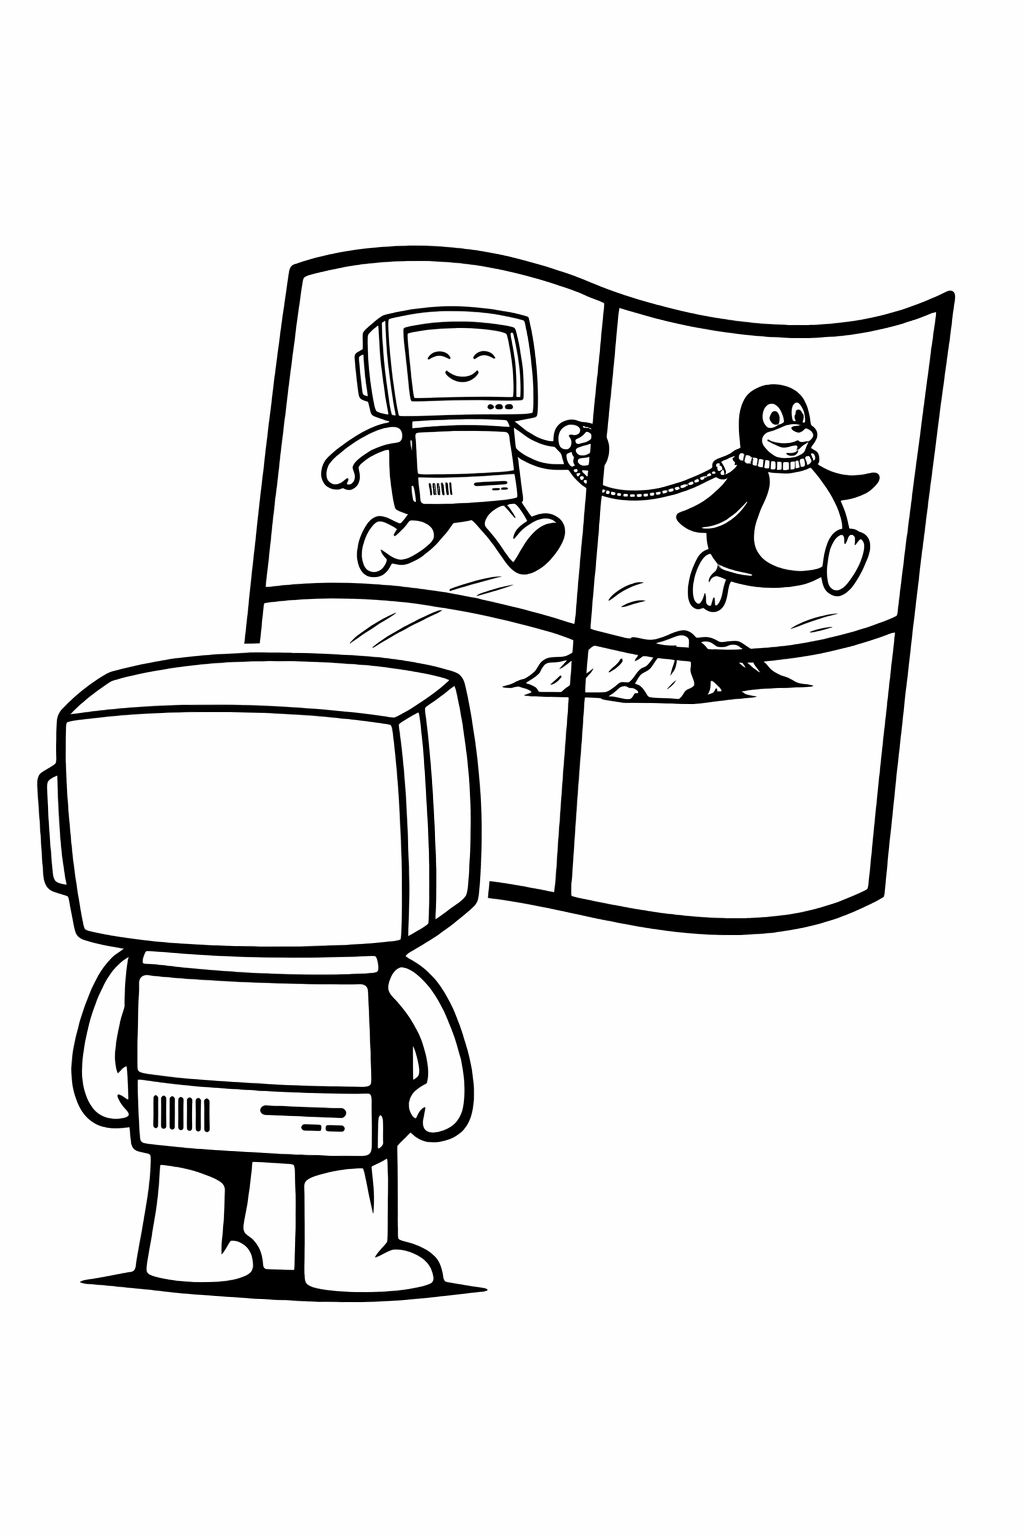
\includegraphics[width=0.38\textwidth]{serivdor_mira_pasear_pinguino_v2}
  \vspace{0.8cm}
\end{center}



\section{Goal (what you will achieve)}
This chapter helps you build the same foundation as Path A, but starting from Windows.

By the end, you will have:
\begin{itemize}[leftmargin=*]
  \item Windows prepared with WSL2 (a real Linux environment inside Windows),
  \item an Ubuntu Linux terminal you can open from the Start menu,
  \item Docker installed and working \emph{via Docker Desktop} (recommended for beginners),
  \item Docker Compose available,
  \item a clean data layout (persistent folders) so containers can be upgraded safely.
\end{itemize}

\section{Who should choose this path?}
Choose \textbf{Path B} if:
\begin{itemize}[leftmargin=*]
  \item you already use Windows and want to start without reinstalling your machine,
  \item you are not comfortable installing Linux directly yet,
  \item you want a gentle, guided learning path.
\end{itemize}

\textbf{Good to know:} this path adds one extra layer (Windows + Linux).
It works well for learning and small self-hosted stacks, but a dedicated Linux server is usually simpler long-term.

\section{Big picture (in plain language)}
\subsection{What is WSL2?}
WSL2 stands for \textbf{Windows Subsystem for Linux 2}. It lets Windows run a real Linux system in the background.

Think of it like this:
\begin{itemize}[leftmargin=*]
  \item Windows is your main computer environment.
  \item WSL2 is a small Linux computer \emph{inside} Windows.
  \item You open an \textbf{Ubuntu app} to get a Linux terminal.
\end{itemize}

\subsection{What is Docker Desktop? (and why we use it here)}
Docker Desktop is the easiest way for beginners to run Docker on Windows.
It integrates with WSL2 so you can run Docker commands from the Ubuntu terminal.

In this manual, \textbf{Path B assumes Docker Desktop}, because it avoids advanced system configuration.

\encourage{Mental model: you type Docker commands in the Ubuntu terminal, but the Docker engine is running in Docker Desktop on Windows. Ubuntu is your control panel; Docker Desktop is the motor.}

\section{Before you start (requirements)}
\begin{itemize}[leftmargin=*]
  \item Windows 10/11 with administrator access.
  \item Internet connection.
  \item Enough disk space (at least 30--50 GB free is a comfortable start).
\end{itemize}

\section{Step 1 --- Install WSL2}
\subsection{1.1 Open PowerShell as Administrator}
\textbf{How:}
\begin{itemize}[leftmargin=*]
  \item Click Start.
  \item Type \texttt{PowerShell}.
  \item Right-click \textbf{Windows PowerShell} and choose \textbf{Run as administrator}.
\end{itemize}

\encourage{This looks more serious than it is. ``Run as administrator'' just gives permission to enable Windows features. You are not breaking anything---you are switching on the Linux subsystem that Windows already supports.}

\subsection{1.2 Install WSL with Ubuntu}
In the admin PowerShell window, run:
\begin{lstlisting}
wsl --install
\end{lstlisting}

\textbf{What this does:}
\begin{itemize}[leftmargin=*]
  \item enables the Windows features required for WSL,
  \item installs WSL2,
  \item installs a default Linux distribution (usually Ubuntu).
\end{itemize}

\textbf{Why you do it:} it creates the Linux environment where we will run server commands.

\subsection{1.3 Reboot if Windows asks you to}
WSL installation often requires a restart.

\subsection{1.4 Confirm WSL2 is active}
Open a normal PowerShell (not necessarily admin) and run:
\begin{lstlisting}
wsl --status
\end{lstlisting}

You want to see that WSL is installed and that the default version is 2.

\paragraph{If needed: set WSL2 as default.}
\begin{lstlisting}
wsl --set-default-version 2
\end{lstlisting}

\section{Step 2 --- Open your Linux terminal (Ubuntu)}
This is the key beginner step: \textbf{your Linux terminal is an app.}

\encourage{If you have never used Linux: perfect. In this path, Linux is just an app you open and close. You can learn it safely, step by step, without reinstalling your computer.}

\subsection{2.1 Open Ubuntu from the Start menu}
\begin{itemize}[leftmargin=*]
  \item Click Start.
  \item Type \texttt{Ubuntu}.
  \item Click the Ubuntu app.
\end{itemize}

A terminal window opens. \textbf{This is Linux.}

\subsection{2.2 Create your Linux username and password}
The first time you open Ubuntu, it will ask you to create:
\begin{itemize}[leftmargin=*]
  \item a Linux username,
  \item a Linux password.
\end{itemize}

\textbf{Important:} this password is for Linux inside WSL, not your Windows password.

\encourage{Two normal things that confuse everyone the first time: (1) this is a new password for Ubuntu, not your Windows password, and (2) when you type it, you will not see any characters on screen. That is normal---type carefully and press Enter.}

\section{Step 3 --- Update Ubuntu inside WSL}
Now that you are in the Ubuntu terminal, run:

\subsection{3.1 Refresh package lists}
\begin{lstlisting}
sudo apt update
\end{lstlisting}
\textbf{What this does:} updates the list of available packages. \\
\textbf{Why you do it:} ensures you install current versions.

\subsection{3.2 Upgrade installed packages}
\begin{lstlisting}
sudo apt upgrade -y
\end{lstlisting}
\textbf{What this does:} upgrades installed software. \\
\textbf{Why you do it:} reduces bugs and security issues.

\subsection{3.3 Install basic tools}
\begin{lstlisting}
sudo apt install -y curl ca-certificates gnupg lsb-release unzip
\end{lstlisting}

\section{Step 4 --- Install Docker (recommended: Docker Desktop)}
On Windows, there are multiple ways to run Docker. For beginners, the best approach is:
\begin{itemize}[leftmargin=*]
  \item install \textbf{Docker Desktop} on Windows,
  \item enable WSL integration,
  \item run Docker commands from the Ubuntu terminal.
\end{itemize}

\subsection{4.1 Install Docker Desktop on Windows}
\textbf{What to do:}
\begin{itemize}[leftmargin=*]
  \item Download and install Docker Desktop (official installer).
  \item During setup, keep the option ``Use WSL 2 instead of Hyper-V'' enabled (recommended).
\end{itemize}

\textbf{Why we do it:} Docker Desktop handles the Windows-side details for you.

\encourage{If the installer offers many options: do not overthink it. The default settings are fine. We only care that Docker Desktop runs and WSL integration is enabled.}

\subsection{4.2 Enable WSL integration}
Open Docker Desktop and go to:
\begin{itemize}[leftmargin=*]
  \item \textbf{Settings} $\rightarrow$ \textbf{Resources} $\rightarrow$ \textbf{WSL Integration}
\end{itemize}

Enable integration for your Ubuntu distribution.

\textbf{What this does:} allows the Ubuntu terminal to use the Docker engine managed by Docker Desktop.

\section{Step 5 --- Verify Docker from the Ubuntu terminal}
In the Ubuntu terminal (WSL), run:

\subsection{5.1 Docker version}
\begin{lstlisting}
docker --version
\end{lstlisting}

\subsection{5.2 Compose version}
\begin{lstlisting}
docker compose version
\end{lstlisting}

\subsection{5.3 Hello-world test}
\begin{lstlisting}
docker run --rm hello-world
\end{lstlisting}

If this works, Docker is correctly installed and integrated.

\encourage{Nice. This is the big milestone. From here on, you are mostly repeating the same pattern: define a service in Compose, start it, and open it in your browser.}

\section{Step 6 --- Create a clean data layout (WSL-friendly)}
We use the same principle: containers are disposable; data must persist.

\subsection{6.1 Create folders inside Linux}
In the Ubuntu terminal:
\begin{lstlisting}
sudo mkdir -p /srv/{docker,photos,music,drive,ai,backups}
sudo mkdir -p /srv/docker/compose
sudo chown -R $USER:$USER /srv
\end{lstlisting}

\textbf{Why inside WSL?} It is faster and more reliable to keep Docker volumes on the Linux filesystem used by WSL.

\subsection{6.2 Important note about Windows drives}
You can access Windows folders from WSL under \texttt{/mnt/c/}, \texttt{/mnt/d/}, etc.
However, for Docker data and databases, using the Linux filesystem (inside WSL) is usually more stable and faster.

\section{Step 7 --- (Optional) Remote access}
If you want to access your services from another device on your network, you have two options:
\begin{itemize}[leftmargin=*]
  \item Use Windows networking (Docker Desktop publishes ports on Windows).
  \item Use a VPN (recommended for access outside your home).
\end{itemize}

\textbf{Beginner advice:} start local first (use your browser on the same PC), then expand to network access once everything works.

\section{Verification checklist}
Before moving on, confirm:
\begin{itemize}[leftmargin=*]
  \item You can open Ubuntu from the Start menu (WSL terminal).
  \item \texttt{docker run --rm hello-world} works inside Ubuntu.
  \item You have \texttt{/srv} created inside WSL.
\end{itemize}

\section{Troubleshooting (common issues)}

\subsection{``wsl is not recognized'' in PowerShell}
WSL is not installed or Windows is too old. Update Windows and try again.

If WSL refuses to install, two common causes are:
\begin{itemize}[leftmargin=*]
  \item Windows is outdated.
  \item Virtualization is disabled in BIOS/UEFI.
\end{itemize}
Update Windows first; if the problem persists, check that virtualization is enabled.

\subsection{Ubuntu asks for a password, but nothing appears when typing}
This is normal: Linux passwords do not show characters while you type. Type carefully and press Enter.

\subsection{Docker command not found inside Ubuntu}
Either Docker Desktop is not installed, or WSL integration is not enabled.
Check Docker Desktop settings and enable integration for Ubuntu.

\subsection{Hello-world fails with permission errors}
Try running once with sudo:
\begin{lstlisting}
sudo docker run --rm hello-world
\end{lstlisting}
If that works, then your user is missing Docker permissions in WSL.
Restart Docker Desktop, close and reopen Ubuntu, and try again.

\section{Next step}
Next, you can install the first service (PhotoPrism) using Docker Compose.
From this point onward, the service chapters are the same for Path A and Path B.

% --- Optional Advanced Notes (append at the end of chapters/02B_server_windows_wsl2_docker.tex) ---

\section{Optional advanced notes (read only if you need them)}
This section is intentionally optional. If your Docker + WSL2 setup works, you can skip it.

\subsection{A) Do I need Docker Desktop? (alternatives)}
For most beginners, \textbf{Docker Desktop is the simplest path} on Windows.
However, there are alternatives:

\begin{itemize}[leftmargin=*]
  \item \textbf{Docker Engine inside WSL2 (without Docker Desktop).}
  This can work, but it requires extra configuration (often systemd support, networking details, and careful permissions).
  \item \textbf{A dedicated Linux machine or Linux VM.}
  This often ends up simpler than fighting Windows-specific quirks if you want a permanent server.
\end{itemize}

\textbf{Recommendation:} Start with Docker Desktop. If you later decide you want a cleaner long-term server,
move to Path A (Linux) using the same Compose files and the same data-layout principles.

\subsection{B) About \texttt{systemctl} and systemd inside WSL2}
On a classic Linux server, services are managed by \texttt{systemd} and the command \texttt{systemctl}.
On WSL2, systemd support depends on your Windows/WSL configuration.

If you run:
\begin{lstlisting}
systemctl status docker
\end{lstlisting}
and it fails, that does \textbf{not} automatically mean Docker is broken.
In the Docker Desktop workflow, Docker is managed by Docker Desktop on Windows, not by systemd inside WSL.

\textbf{What to do instead:}
\begin{itemize}[leftmargin=*]
  \item open Docker Desktop and confirm it is running,
  \item in Ubuntu, run \texttt{docker ps} to see whether Docker responds.
\end{itemize}

\subsection{C) Where should I store data on Windows + WSL2?}
You can store files in:
\begin{itemize}[leftmargin=*]
  \item the Linux filesystem (inside WSL): e.g., \texttt{/srv/...}
  \item Windows drives mounted into WSL: e.g., \texttt{/mnt/c/...}, \texttt{/mnt/d/...}
\end{itemize}

\textbf{Practical rule:}
\begin{itemize}[leftmargin=*]
  \item For Docker volumes, databases, and indexes: prefer the Linux filesystem (\texttt{/srv}) for performance and fewer permission issues.
  \item For large media archives you already have on Windows disks: you can mount/read them from \texttt{/mnt/d/...}, but test performance.
\end{itemize}

\subsection{D) Accessing your services from another device}
In most Docker Desktop setups, when you publish a port (e.g., \texttt{8080:8080}),
Windows exposes that port on your local network interface.

\textbf{Typical workflow:}
\begin{itemize}[leftmargin=*]
  \item First test locally: open your browser on the same PC and use \texttt{http://localhost:PORT}.
  \item Then test from another device on the same network: use \texttt{http://WINDOWS\_IP:PORT}.
\end{itemize}

If it does not work from another device:
\begin{itemize}[leftmargin=*]
  \item check the Windows firewall rules,
  \item ensure Docker Desktop is running,
  \item verify the container really publishes the port (\texttt{docker ps} shows port mappings).
\end{itemize}

\subsection{E) WSL2 resource limits (CPU/RAM/disk)}
WSL2 uses Windows resources. On some systems, you may want to limit its maximum RAM/CPU usage,
especially if your laptop becomes slow.

This can be configured via a \texttt{.wslconfig} file in your Windows user home directory.
If you do not have performance problems, ignore this.
If you do, this is a good first tuning knob.

\subsection{F) Backups on Windows + WSL2 (simple advice)}
Even in a beginner setup, plan backups early:
\begin{itemize}[leftmargin=*]
  \item keep your persistent folders under a single root (we use \texttt{/srv}),
  \item periodically copy that folder to an external drive or another machine.
\end{itemize}

\textbf{Important:} if you store your Docker data in the Linux filesystem inside WSL,
make sure your backup method can access it reliably (e.g., exporting/copying from inside the Ubuntu terminal). 
% chapters/04_theory_compose_yaml.tex
\chapter{How to read this manual: YAML and Docker Compose (just enough theory)}
\label{ch:theory_compose_yaml}


\begin{center}
  \vspace{0.6cm}
  
\includegraphics[width=0.38\textwidth]{serivdor_estudia}
  \vspace{0.8cm}
\end{center}


\section{Goal (what you will achieve)}
This chapter gives you the minimum theory needed to follow the rest of the manual confidently.

By the end, you will:
\begin{itemize}[leftmargin=*]
  \item understand what a \texttt{docker-compose.yml} file is and why we use it,
  \item recognize the most common YAML patterns (indentation, lists, key/value),
  \item know what \texttt{services}, \texttt{ports}, \texttt{volumes}, and \texttt{environment} mean,
  \item understand what \texttt{.env} is and why we keep passwords there,
  \item know what MariaDB is and when you need a database,
  \item avoid the most common beginner mistakes (especially indentation and permissions).
\end{itemize}

\encourage{If YAML looks like mysterious hieroglyphs: that is normal. After this chapter, you will be able to read Compose files like a recipe. You do not need to become a chef.}

\section{What is YAML?}
YAML is a human-friendly text format used to describe structured information.
In this manual, we use YAML because Docker Compose uses it.

\subsection*{Three rules that explain 90\% of YAML}
\begin{enumerate}[leftmargin=*]
  \item \textbf{Indentation matters.} YAML uses spaces to show hierarchy.
  \item \textbf{Key: value} pairs define settings.
  \item \textbf{Lists use dashes} (\texttt{- item}).
\end{enumerate}

\subsection*{Example: key/value and indentation}
\begin{lstlisting}
person:
  name: Mattia
  role: Admin
\end{lstlisting}
Here, \texttt{name} and \texttt{role} belong ``inside'' \texttt{person} because they are indented.

\subsection*{Example: a list}
\begin{lstlisting}
shopping_list:
  - pasta
  - tomatoes
  - coffee
\end{lstlisting}

\subsection*{What does \texttt{\#} mean?}
A \texttt{\#} starts a \textbf{comment}. Comments are ignored by the computer.
They are there for humans.

\begin{lstlisting}
# This is a comment. It does nothing, but it helps you understand the file.
\end{lstlisting}

\encourage{YAML is picky, but not evil. If something breaks, the most common cause is indentation (missing spaces), not your life choices.}

\section{What is Docker Compose (in plain language)?}
Docker Compose is a tool that reads a file called \texttt{docker-compose.yml} and starts a set of containers for you.

Think of it like a playlist:
\begin{itemize}[leftmargin=*]
  \item the file lists which services you want (PhotoPrism, Navidrome, etc.),
  \item Compose starts them in a consistent way,
  \item you can stop them, restart them, and upgrade them reliably.
\end{itemize}

\subsection*{Why we use Compose in this manual}
Without Compose, you would type long Docker commands every time.
With Compose, the setup becomes:
\begin{itemize}[leftmargin=*]
  \item \textbf{reproducible} (you can move it to another machine),
  \item \textbf{documented} (the file explains what you run),
  \item \textbf{upgrade-friendly} (pull new images and restart).
\end{itemize}

\section{A Compose file is a ``service recipe''}
Most of our Compose files follow the same pattern:

\begin{lstlisting}
services:
  some-service:
    image: some/image:tag
    ports:
      - "1234:1234"
    environment:
      KEY: "value"
    volumes:
      - /host/path:/container/path
\end{lstlisting}

Let's translate the important words.

\section{Core blocks you will see everywhere}
\subsection{\texttt{services}}
A \texttt{service} is one container (or sometimes a group of containers with one role).
In our manual:
\begin{itemize}[leftmargin=*]
  \item PhotoPrism is a service,
  \item MariaDB (database) is another service,
  \item Navidrome is a service,
  \item Ollama and Open WebUI are services.
\end{itemize}

\subsection{\texttt{image}}
\texttt{image} tells Docker what software to run.
\begin{itemize}[leftmargin=*]
  \item An \textbf{image} is like a packaged application template.
  \item A \textbf{container} is a running instance of that image.
\end{itemize}

Example:
\begin{lstlisting}
image: photoprism/photoprism:latest
\end{lstlisting}

\subsection{\texttt{ports}}
Ports let your browser or apps reach a service.

Example:
\begin{lstlisting}
ports:
  - "2342:2342"
\end{lstlisting}

\textbf{How to read it:}
\begin{itemize}[leftmargin=*]
  \item left side = host (your machine) port,
  \item right side = container port (inside the service).
\end{itemize}

So \texttt{"2342:2342"} means:
\begin{itemize}[leftmargin=*]
  \item open port 2342 on your machine,
  \item forward it to port 2342 inside the container.
\end{itemize}

\subsection{\texttt{volumes}}
Volumes are the most important concept for data safety.

Example:
\begin{lstlisting}
volumes:
  - /srv/photos/originals:/photoprism/originals
\end{lstlisting}

\textbf{How to read it:}
\begin{itemize}[leftmargin=*]
  \item left side = real folder on your disk (persistent),
  \item right side = folder inside the container (where the app expects files).
\end{itemize}

\textbf{Why it matters:}
\begin{itemize}[leftmargin=*]
  \item You can delete/recreate containers without losing data.
  \item Backups become simple: you back up \texttt{/srv/...}.
\end{itemize}

\encourage{Repeat this mantra: containers are disposable; data is not. If you get volumes right, you win.}

\subsection{\texttt{environment}}
Environment variables are configuration settings given to the application.

Example:
\begin{lstlisting}
environment:
  PHOTOPRISM_ADMIN_PASSWORD: "a-strong-password"
\end{lstlisting}

\textbf{Why we use them:}
\begin{itemize}[leftmargin=*]
  \item They keep configuration close to the Compose file.
  \item They are the standard way many containers are configured.
\end{itemize}

\section{What is a \texttt{.env} file (and why we use it)?}
A \texttt{.env} file sits next to \texttt{docker-compose.yml} and stores variables.

Example:
\begin{lstlisting}
PHOTOPRISM_ADMIN_PASSWORD=CHANGE_THIS
MARIADB_PASSWORD=CHANGE_THIS_TOO
\end{lstlisting}

Then, in YAML, we reference them like:
\begin{lstlisting}
PHOTOPRISM_ADMIN_PASSWORD: ${PHOTOPRISM_ADMIN_PASSWORD}
\end{lstlisting}

\textbf{Why we do it:}
\begin{itemize}[leftmargin=*]
  \item keeps passwords out of the YAML (cleaner),
  \item makes it easier to share Compose files without leaking secrets,
  \item centralizes configuration in one place.
\end{itemize}

\section{What is MariaDB, and why does PhotoPrism need it?}
MariaDB is a database server (similar to MySQL).
A database is a structured storage system for:
\begin{itemize}[leftmargin=*]
  \item indexes,
  \item metadata,
  \item search tables,
  \item application state.
\end{itemize}

Some apps can store everything in simple files; others work better with a database.
PhotoPrism can use SQLite or MySQL/MariaDB, but for larger libraries and better performance, MariaDB is commonly used.

\section{Useful words you will see later (and what they mean)}
This manual tries to stay beginner-friendly, but some technical words are unavoidable.
Here are the ones that appear in later chapters, explained in plain language.

\subsection{MySQL vs MariaDB}
\textbf{MySQL} and \textbf{MariaDB} are very similar database servers.
MariaDB started as a community-developed alternative to MySQL and is widely used.
In practice, many applications treat them as interchangeable for common use.

\textbf{What matters for you:}
\begin{itemize}[leftmargin=*]
  \item The ``database service'' is the container that stores structured data (metadata, indexes, users, settings).
  \item When a config says \texttt{DB\_HOST} or \texttt{MYSQL\_HOST}, it means: \emph{the name of the database service on the Docker network}.
\end{itemize}

Example:
\begin{lstlisting}
MYSQL_HOST: db
\end{lstlisting}
This means: ``connect to the container named \texttt{db} (service name), not to an external server.''

\subsection{Redis and Memcached (fast helpers)}
\textbf{Redis} and \textbf{Memcached} are small services used as memory caches.
They help performance and reduce database load.

In this manual:
\begin{itemize}[leftmargin=*]
  \item Nextcloud uses Redis for locking/caching (helps stability, especially with many files).
  \item Seafile often uses Memcached for performance.
\end{itemize}

You do not ``use'' them directly as a user; they are internal helpers.

\subsection{Cron and ``background jobs''}
Some apps need periodic tasks: cleanup, indexing, sending notifications, updating shares, etc.
This is often called \textbf{background jobs}.

In Nextcloud, running background jobs properly matters a lot.
That is why we include a dedicated \texttt{cron} container.

\subsection{HTTP vs HTTPS (TLS): the safety layer}
\textbf{HTTP} is plain web traffic. \textbf{HTTPS} is encrypted web traffic (HTTP + TLS).

\textbf{Practical rule:}
\begin{itemize}[leftmargin=*]
  \item On your local network (LAN) and especially when using VPN, HTTP is often acceptable for beginners.
  \item If you expose services to the public internet, you must use HTTPS (TLS) and a proper reverse proxy.
\end{itemize}

\encourage{If you are unsure: do not expose your services publicly yet. Use VPN first. It is safer and simpler.}

\subsection{Domains, hostnames, and ``trusted domains''}
A \textbf{hostname} is a human-friendly name for a machine (e.g., \texttt{server}, \texttt{nextcloud}).
A \textbf{domain} is a public name you can buy (e.g., \texttt{yourname.com}).

\textbf{Trusted domains} are a security feature in apps like Nextcloud:
they refuse requests from unknown hostnames to prevent certain attacks.
That is why you must list the addresses you use (e.g., \texttt{localhost}, \texttt{SERVER\_IP}, or your domain).

\subsection{UID/GID (why permissions sometimes hurt)}
Linux permissions are based on user IDs:
\begin{itemize}[leftmargin=*]
  \item \textbf{UID}: user ID
  \item \textbf{GID}: group ID
\end{itemize}

Some containers run as a specific internal user. If file permissions do not match, you may see ``permission denied'' errors.
That is why some services support setting \texttt{UID/GID} explicitly.

\subsection{JWT (a shared secret for trusted communication)}
\textbf{JWT} stands for JSON Web Token. In our context, you do not need to learn the standard.
You only need the practical meaning:

\begin{itemize}[leftmargin=*]
  \item Some integrations (like OnlyOffice) require a \textbf{shared secret}.
  \item Both services must use the \emph{same secret} to trust each other.
  \item This is often configured as \texttt{JWT\_SECRET}.
\end{itemize}

\textbf{Practical rule:} choose a long random string and keep it consistent across the services that need it.

\subsection{Reverse proxy (optional, advanced)}
A \textbf{reverse proxy} is a gateway in front of your services.
It can:
\begin{itemize}[leftmargin=*]
  \item route traffic to the correct container,
  \item provide HTTPS/TLS,
  \item centralize security headers and access rules.
\end{itemize}

We do not require a reverse proxy in this manual, because it is optional and adds complexity.
If you later want public access with a domain, a reverse proxy becomes important.

\section{Finding your server address (IP): the one thing you need for mobile access}
Many chapters say: open \texttt{http://SERVER\_IP:PORT}.
This section explains what \texttt{SERVER\_IP} means and how to find it.

\subsection*{What is \texttt{SERVER\_IP}?}
It is the local network address of the machine running your services (PhotoPrism, Navidrome, etc.).
If your phone is on the same Wi-Fi, it can reach that address directly.

\encourage{You do not need to understand networking deeply. You only need to find the IP once, then reuse it everywhere.}

\subsection{Linux (Path A)}
In a Linux terminal, run one of these:

\begin{lstlisting}
hostname -I
\end{lstlisting}

or:

\begin{lstlisting}
ip a
\end{lstlisting}

Look for an address like \texttt{192.168.x.x} or \texttt{10.x.x.x}. That is usually your LAN IP.

\subsection{Windows (Path B)}
Open PowerShell and run:

\begin{lstlisting}
ipconfig
\end{lstlisting}

Look for \texttt{IPv4 Address} under your active network adapter (Wi-Fi or Ethernet).

\subsection{Quick sanity check}
From another device on the same Wi-Fi (phone/tablet/laptop), open a browser and try:

\begin{lstlisting}
http://SERVER_IP:2342
\end{lstlisting}

If PhotoPrism loads, you found the right IP.

\subsection*{Common confusion: multiple IP addresses}
Sometimes you will see more than one IP address (Ethernet + Wi-Fi + VPN).
Use the one that matches the network you are currently using (for example, the Wi-Fi subnet).


\section{VPN: the safe way to access your server from outside}
Sooner or later you will want to access your services when you are not at home (or not on the same Wi-Fi).
There are two broad approaches:
\begin{itemize}[leftmargin=*]
  \item \textbf{Expose services publicly} (open ports on the router, set up a domain, reverse proxy, TLS).
  \item \textbf{Use a VPN} (recommended for beginners).
\end{itemize}

\subsection{What is a VPN (plain language)?}
A VPN (Virtual Private Network) creates an encrypted ``tunnel'' between your device (phone/laptop) and your home network (or server).
When connected, your device behaves \emph{as if it were inside your home network}.
That means:
\begin{itemize}[leftmargin=*]
  \item you can use the same addresses as at home, e.g., \texttt{http://SERVER\_IP:2342},
  \item you do not need to expose every service to the public internet.
\end{itemize}

\subsection{Why this manual prefers VPN first}
Public exposure can be done safely, but it has more moving parts and more ways to misconfigure things.
A VPN is often:
\begin{itemize}[leftmargin=*]
  \item simpler,
  \item safer by default,
  \item easier to reason about (``only my devices can enter'').
\end{itemize}


\encourage{If your goal is ``access my stuff from anywhere'', a VPN is usually the shortest path that does not turn into a security project.}

\subsection{How VPN fits into this manual}
Our default workflow is:
\begin{itemize}[leftmargin=*]
  \item \textbf{Local first:} make everything work on your local network (LAN/Wi-Fi).
  \item \textbf{Then remote:} add a VPN so you can access the same services while travelling.
\end{itemize}

\subsection{Do we teach VPN setup here?}
We give the concept here to avoid confusion, but a full VPN setup depends on your environment
(router, ISP restrictions, CGNAT, existing university VPN, etc.).

For that reason, the step-by-step VPN setup is placed in a separate optional appendix:
Appendix~\ref{app:vpn}.

\section{Common beginner mistakes (and how to avoid them)}
\subsection{Mistake 1: indentation errors in YAML}
If Compose fails with a YAML parsing error:
\begin{itemize}[leftmargin=*]
  \item check that indentation uses spaces (not tabs),
  \item check that lists use \texttt{- } and align correctly,
  \item when in doubt, compare to a known working example from this manual.
\end{itemize}

\subsection{Mistake 2: editing the wrong file in the wrong folder}
When we say:
\begin{lstlisting}
cd /srv/docker/compose/photoprism
\end{lstlisting}
we mean: \textbf{go into that folder first}, then run Compose there.
Otherwise, Docker might run a different project than you think.

\subsection{Mistake 3: storing data inside the container}
If your \texttt{volumes:} are missing or wrong, your data may disappear when the container is recreated.
Always check that important folders map to \texttt{/srv/...} on the host.

\subsection{Mistake 4: confusing host ports and container ports}
If you map \texttt{"1234:2342"}, you must open \texttt{http://localhost:1234} in your browser.
The left side is the port you use from outside.

\subsection{Mistake 5: permission issues on mounted folders}
If an app cannot write to a volume:
\begin{itemize}[leftmargin=*]
  \item ensure the folder exists,
  \item ensure your user owns it (or the container is configured with matching UID/GID),
  \item on Linux, a common fix is:
\end{itemize}

\begin{lstlisting}
sudo chown -R $USER:$USER /srv
\end{lstlisting}

\section{The three Compose commands you will use all the time}
\subsection*{Start services}
\begin{lstlisting}
docker compose up -d
\end{lstlisting}

\subsection*{Stop services}
\begin{lstlisting}
docker compose down
\end{lstlisting}

\subsection*{See what is running}
\begin{lstlisting}
docker ps
\end{lstlisting}

\subsection*{Read logs (your best friend when things fail)}
\begin{lstlisting}
docker compose logs -f --tail=100
\end{lstlisting}

\encourage{When something fails: do not guess. Check logs. Logs look intimidating, but they usually contain the exact clue you need.}

\section{Next step}
Now you can read the Compose files in the service chapters like a recipe.
In Appendix B, you will also find all Compose files collected in one place for easy copy/paste. 
% Service chapters (uncomment as you write them)
 % chapters/03_photoprism.tex
\chapter{PhotoPrism: your private photo library}
\label{ch:photoprism}


\begin{center}
  \vspace{0.6cm}
  
\includegraphics[width=0.38\textwidth]{serivdor_foto_v4}
  \vspace{0.8cm}
\end{center}


\section{Goal (what you will achieve)}
In this chapter you will install PhotoPrism, a self-hosted photo management app that helps you:
\begin{itemize}[leftmargin=*]
  \item browse your photo archive from any browser on your network,
  \item import and index photos without handing them to a third party,
  \item search, tag, and organize your library with modern features.
\end{itemize}

\encourage{This chapter is where the project starts to feel real. Once PhotoPrism opens in your browser, you are no longer ``installing Docker''---you are building your own digital home.}

\section{What is PhotoPrism (plain language)}
PhotoPrism is a web app you host yourself. It scans your photo folders, builds an index, and lets you browse and search your library from a clean web interface.
It runs well in Docker, and the recommended way to run it is with Docker Compose. :contentReference[oaicite:1]{index=1}

\section{Prerequisites}
\begin{itemize}[leftmargin=*]
  \item Docker and Docker Compose working (Chapter 2 or 3).
  \item A folder where your photos will live (we use \texttt{/srv/photos}).
  \item A bit of patience for the first indexing (it can take time on large libraries).
\end{itemize}

\section{Folder layout (what goes where)}
We will keep things simple and predictable:

\begin{itemize}[leftmargin=*]
  \item \texttt{/srv/photos/originals} --- your original photo/video files (the important part!)
  \item \texttt{/srv/photos/import} --- optional folder for importing new files into PhotoPrism
  \item \texttt{/srv/photos/storage} --- PhotoPrism internal storage (thumbnails, index, cache)
  \item \texttt{/srv/docker/compose/photoprism} --- Compose file and environment file
\end{itemize}

Create folders (Linux path; on WSL2, run the same inside Ubuntu):

\begin{lstlisting}
mkdir -p /srv/docker/compose/photoprism
mkdir -p /srv/photos/{originals,import,storage,mariadb}
\end{lstlisting}

\encourage{Do not store your originals inside the container. Keep them in /srv/photos/originals so you can back them up and move them whenever you want.}

\section{Step 1 --- Create the Compose project}
Go to the PhotoPrism Compose folder:

\begin{lstlisting}
cd /srv/docker/compose/photoprism
\end{lstlisting}

\subsection{1.1 Create an environment file}
Create \texttt{.env} (this keeps passwords out of the YAML):

\begin{lstlisting}
nano .env
\end{lstlisting}

Paste and edit:

\begin{lstlisting}
# --- PhotoPrism admin login ---
PHOTOPRISM_ADMIN_USER=admin
PHOTOPRISM_ADMIN_PASSWORD=CHANGE_THIS_TO_A_LONG_PASSWORD

# --- Database (MariaDB) ---
MARIADB_DATABASE=photoprism
MARIADB_USER=photoprism
MARIADB_PASSWORD=CHANGE_THIS_DB_PASSWORD
MARIADB_ROOT_PASSWORD=CHANGE_THIS_ROOT_PASSWORD

# --- Optional: match your Linux user (helps avoid permission issues) ---
# On Linux, these can often be left as-is if your user is UID/GID 1000.
# On Windows/macOS, setting them explicitly can help if you see permission errors.
PHOTOPRISM_UID=1000
PHOTOPRISM_GID=1000
\end{lstlisting}

\textbf{Why this matters:}
\begin{itemize}[leftmargin=*]
  \item PhotoPrism needs an admin password.
  \item MariaDB needs credentials.
  \item Keeping secrets in \texttt{.env} is cleaner and safer than hardcoding them in YAML.
\end{itemize}

\encourage{Yes, set real passwords. Future-you will thank present-you.}

\subsection{1.2 Create \texttt{docker-compose.yml}}
Create the Compose file:

\begin{lstlisting}
nano docker-compose.yml
\end{lstlisting}

Paste:

\begin{lstlisting}
services:
  mariadb:
    image: mariadb:11
    container_name: photoprism-mariadb
    restart: unless-stopped
    environment:
      MARIADB_DATABASE: ${MARIADB_DATABASE}
      MARIADB_USER: ${MARIADB_USER}
      MARIADB_PASSWORD: ${MARIADB_PASSWORD}
      MARIADB_ROOT_PASSWORD: ${MARIADB_ROOT_PASSWORD}
    volumes:
      - /srv/photos/mariadb:/var/lib/mysql

  photoprism:
    image: photoprism/photoprism:latest
    container_name: photoprism
    restart: unless-stopped
    depends_on:
      - mariadb
    ports:
      - "2342:2342"
    environment:
      PHOTOPRISM_ADMIN_USER: ${PHOTOPRISM_ADMIN_USER}
      PHOTOPRISM_ADMIN_PASSWORD: ${PHOTOPRISM_ADMIN_PASSWORD}

      # Database config (PhotoPrism supports sqlite or mysql; MariaDB uses mysql driver)
      PHOTOPRISM_DATABASE_DRIVER: "mysql"
      PHOTOPRISM_DATABASE_SERVER: "mariadb:3306"
      PHOTOPRISM_DATABASE_NAME: ${MARIADB_DATABASE}
      PHOTOPRISM_DATABASE_USER: ${MARIADB_USER}
      PHOTOPRISM_DATABASE_PASSWORD: ${MARIADB_PASSWORD}

      # File permissions (often helps on Linux; may be useful on Windows/macOS too)
      PHOTOPRISM_UID: ${PHOTOPRISM_UID}
      PHOTOPRISM_GID: ${PHOTOPRISM_GID}

      # Optional quality-of-life settings:
      PHOTOPRISM_SITE_URL: "http://localhost:2342/"
      PHOTOPRISM_ORIGINALS_LIMIT: 5000

    volumes:
      - /srv/photos/originals:/photoprism/originals
      - /srv/photos/import:/photoprism/import
      - /srv/photos/storage:/photoprism/storage
\end{lstlisting}

\textbf{Notes:}
\begin{itemize}[leftmargin=*]
  \item PhotoPrism’s default port is \texttt{2342}. :contentReference[oaicite:2]{index=2}
  \item Database variables follow PhotoPrism config options for MySQL/MariaDB. :contentReference[oaicite:3]{index=3}
\end{itemize}

\encourage{If YAML feels fragile: it is. Indentation matters. If something fails, it is usually one missing space, not a life problem.}

\section{Step 2 --- Start PhotoPrism}
Start the stack:

\begin{lstlisting}
docker compose up -d
\end{lstlisting}

Check containers:

\begin{lstlisting}
docker ps
\end{lstlisting}

\subsection{View logs (first debugging tool)}
If something does not start:

\begin{lstlisting}
docker compose logs -f --tail=100
\end{lstlisting}

\section{Step 3 --- Open PhotoPrism in your browser}
On the same machine:
\begin{lstlisting}
http://localhost:2342
\end{lstlisting}

From another device on the same network:
\begin{lstlisting}
http://SERVER_IP:2342
\end{lstlisting}

Log in with the admin user/password from your \texttt{.env} file.

\encourage{If the login page loads: you are already winning. Most ``server projects'' fail before this moment.}

\encourage{If it works on \texttt{localhost} but not from your phone, the usual culprit is the firewall (especially on Windows). This is normal -- see the ``Access from mobile'' section and the VPN appendix (Appendix~\ref{app:vpn}).}

\section{Step 4 --- Add photos and index}
\subsection{Option A: put files directly in originals}
Copy photos into:
\begin{lstlisting}
/srv/photos/originals
\end{lstlisting}

Then in PhotoPrism, use the web interface to index (or re-index) the library.

\subsection{Option B: use the import folder}
Copy files into:
\begin{lstlisting}
/srv/photos/import
\end{lstlisting}

Then use PhotoPrism’s import workflow in the UI.

\section{Verification checklist}
You are done when:
\begin{itemize}[leftmargin=*]
  \item \texttt{docker ps} shows \texttt{photoprism} and \texttt{photoprism-mariadb} running,
  \item \texttt{http://localhost:2342} loads the PhotoPrism login page,
  \item you can log in and see the PhotoPrism dashboard,
  \item after adding photos, indexing completes and photos appear.
\end{itemize}

\section{Common pitfalls (and quick fixes)}
\subsection{1) ``Cannot connect to database''}
Usually the database is not ready yet, or credentials do not match.
\begin{itemize}[leftmargin=*]
  \item Check logs: \texttt{docker compose logs -f --tail=100}
  \item Ensure \texttt{PHOTOPRISM\_DATABASE\_*} matches the MariaDB variables in \texttt{.env}.
  \item Restart after fixes: \texttt{docker compose down} then \texttt{docker compose up -d}
\end{itemize}
PhotoPrism troubleshooting notes commonly point to network/database connectivity and correct host/port. :contentReference[oaicite:4]{index=4}

\subsection{2) Permission problems on mounted folders}
Symptoms: PhotoPrism cannot write to \texttt{/photoprism/storage} or fails creating files.
\begin{itemize}[leftmargin=*]
  \item Make sure \texttt{/srv/photos/storage} exists and is writable.
  \item On Linux, run: \texttt{sudo chown -R \$USER:\$USER /srv/photos}
  \item If needed, set \texttt{PHOTOPRISM\_UID} and \texttt{PHOTOPRISM\_GID} explicitly. :contentReference[oaicite:5]{index=5}
\end{itemize}

\subsection{3) ``It is slow'' on first run}
The first indexing generates thumbnails and builds the database. This is normal.
\begin{itemize}[leftmargin=*]
  \item Let it run.
  \item Keep the machine on.
  \item Consider indexing overnight for large libraries.
\end{itemize}
\encourage{Slow is not broken. The first scan is the hardest; later updates are much faster.}

\subsection{4) Wrong URL/port}
Default is \texttt{http} on port \texttt{2342}. :contentReference[oaicite:6]{index=6}
\begin{itemize}[leftmargin=*]
  \item Local: \texttt{http://localhost:2342}
  \item Network: \texttt{http://SERVER\_IP:2342}
\end{itemize}

\subsection{5) Exposing PhotoPrism to the public internet too early}
Do not expose PhotoPrism publicly until you understand reverse proxies and TLS.
Start with LAN or VPN access. (We keep public exposure optional in this manual.)

\section{Access from mobile and tablet}
You do not need a special app to use PhotoPrism. A browser is enough.

\subsection*{On the same Wi-Fi (local network)}
\begin{itemize}[leftmargin=*]
  \item Find the IP address of the machine running PhotoPrism (the ``server'').
  \item On your phone/tablet browser, open:
\end{itemize}

\begin{lstlisting}
http://SERVER_IP:2342
\end{lstlisting}

\subsection*{Outside your home (recommended: VPN)}
If you want access while travelling, the safest beginner approach is:
\begin{itemize}[leftmargin=*]
  \item connect your phone to your VPN,
  \item then use the same address:
\end{itemize}

\begin{lstlisting}
http://SERVER_IP:2342
\end{lstlisting}

\encourage{Start with local Wi-Fi first. Once it works locally, adding VPN access is usually just one extra step, not a whole new project.}

\subsection*{Make it feel like an app (Add to Home Screen)}
Most browsers let you add the PhotoPrism page to your home screen.
This creates an icon and opens it in an ``app-like'' full-screen mode.
Look for \textbf{Share} $\rightarrow$ \textbf{Add to Home Screen} (wording may vary).


\section{Next step}
Next, we install Navidrome (music server). It is simpler than PhotoPrism:
one container, one library folder, one web UI. 
% chapters/06_navidrome.tex
\chapter{Navidrome: your private music server}
\label{ch:navidrome}

\begin{center}
  \vspace{0.6cm}
  
\includegraphics[width=0.38\textwidth]{serivdor_musica_v2}
  \vspace{0.8cm}
\end{center}



\section{Goal (what you will achieve)}
In this chapter you will install Navidrome, a lightweight self-hosted music server.
By the end, you will have:
\begin{itemize}[leftmargin=*]
  \item a web music library you can access from a browser on your network,
  \item a clean folder layout for your music files and Navidrome data,
  \item a simple Compose setup you can start/stop/upgrade reliably.
\end{itemize}

\encourage{This one is a morale boost: Navidrome is usually fast to deploy and feels instantly useful.}

\section{What is Navidrome (plain language)}
Navidrome is a music streaming server you run yourself. You point it to your music folder,
it builds an index, and it serves a modern web UI. It also supports Subsonic-compatible clients
(many mobile apps can connect to it), but you can start with the browser and keep it simple.

\section{Prerequisites}
\begin{itemize}[leftmargin=*]
  \item Docker and Docker Compose working (Chapters 2A or 2B).
  \item A folder with your music library (we use \texttt{/srv/music/library}).
\end{itemize}

\section{Folder layout}
We will use:
\begin{itemize}[leftmargin=*]
  \item \texttt{/srv/music/library} --- your music files (the important part)
  \item \texttt{/srv/music/data} --- Navidrome database and cache (persistent)
  \item \texttt{/srv/docker/compose/navidrome} --- Compose files
\end{itemize}

Create folders (Linux path; on WSL2, run inside Ubuntu):

\begin{lstlisting}
mkdir -p /srv/docker/compose/navidrome
mkdir -p /srv/music/{library,data}
\end{lstlisting}

\encourage{Same principle as always: your music lives on disk (\texttt{/srv/music/library}), not ``inside Docker''.}

\section{Step 1 --- Create the Compose project}
Go to the Navidrome compose folder:

\begin{lstlisting}
cd /srv/docker/compose/navidrome
\end{lstlisting}

\subsection{1.1 Create a simple environment file (recommended)}
Create \texttt{.env}:

\begin{lstlisting}
nano .env
\end{lstlisting}

Paste (you can keep defaults for now):

\begin{lstlisting}
# --- Navidrome basics ---
ND_SCANSCHEDULE=1h
ND_LOGLEVEL=info

# --- Optional: set timezone for correct timestamps ---
TZ=Europe/Madrid
\end{lstlisting}

\textbf{What this does:}
\begin{itemize}[leftmargin=*]
  \item \texttt{ND\_SCANSCHEDULE} tells Navidrome how often to scan for new files,
  \item \texttt{TZ} helps with correct time display and logs.
\end{itemize}

\subsection{1.2 Create \texttt{docker-compose.yml}}
Create the Compose file:

\begin{lstlisting}
nano docker-compose.yml
\end{lstlisting}

Paste:

\begin{lstlisting}
services:
  navidrome:
    image: deluan/navidrome:latest
    container_name: navidrome
    restart: unless-stopped
    ports:
      - "4533:4533"
    environment:
      ND_SCANSCHEDULE: ${ND_SCANSCHEDULE}
      ND_LOGLEVEL: ${ND_LOGLEVEL}
      TZ: ${TZ}
    volumes:
      - /srv/music/data:/data
      - /srv/music/library:/music:ro
\end{lstlisting}

\textbf{How to read it:}
\begin{itemize}[leftmargin=*]
  \item Port \texttt{4533} will be the web UI.
  \item \texttt{/srv/music/data} stores Navidrome's database (persistent).
  \item \texttt{/srv/music/library} is mounted as \texttt{:ro} (read-only) to protect your originals.
\end{itemize}

\encourage{Mounting the music folder as read-only is a nice beginner safety belt: the server can index and stream, but it cannot accidentally modify your files.}

\section{Step 2 --- Start Navidrome}
Start the container:

\begin{lstlisting}
docker compose up -d
\end{lstlisting}

Check status:

\begin{lstlisting}
docker ps
\end{lstlisting}

If something looks wrong, check logs:

\begin{lstlisting}
docker compose logs -f --tail=100
\end{lstlisting}

\section{Step 3 --- Open Navidrome in your browser}
On the same machine:
\begin{lstlisting}
http://localhost:4533
\end{lstlisting}

From another device on the same network:
\begin{lstlisting}
http://SERVER_IP:4533
\end{lstlisting}

\subsection{First login}
On the first run, Navidrome typically asks you to create an admin user in the web UI.

\encourage{If you see the login/setup screen: you are done with the hard part. From here it is just adding music.}

\section{Step 4 --- Add music and let it scan}
Copy your music into:
\begin{lstlisting}
/srv/music/library
\end{lstlisting}

Navidrome will scan automatically according to \texttt{ND\_SCANSCHEDULE}.
If you add a lot of files, give it some time to index them.

\section{Verification checklist}
You are done when:
\begin{itemize}[leftmargin=*]
  \item \texttt{docker ps} shows \texttt{navidrome} running,
  \item \texttt{http://localhost:4533} loads the Navidrome UI,
  \item you can create/login to the admin user,
  \item after adding music, albums and tracks appear.
\end{itemize}

\section{Common pitfalls (and quick fixes)}
\subsection{1) No music appears}
Most common causes:
\begin{itemize}[leftmargin=*]
  \item The library folder is empty, or you copied files to the wrong path.
  \item The container cannot see your files because the volume path is wrong.
\end{itemize}

Quick checks:
\begin{itemize}[leftmargin=*]
  \item Confirm your files are in \texttt{/srv/music/library} on the host.
  \item Confirm the container mount exists:
\end{itemize}

\begin{lstlisting}
docker exec -it navidrome ls -la /music | head
\end{lstlisting}

\subsection{2) Permission problems}
Because we mount the music library read-only, permission issues are usually about the data folder:
\begin{itemize}[leftmargin=*]
  \item Ensure \texttt{/srv/music/data} exists.
  \item Ensure it is writable by your user (and thus by Docker):
\end{itemize}

\begin{lstlisting}
sudo chown -R $USER:$USER /srv/music
\end{lstlisting}

\subsection{3) Port already in use}
If port 4533 is already used by another service, change the left side of the port mapping.

Example: use port 4534 on the host:
\begin{lstlisting}
ports:
  - "4534:4533"
\end{lstlisting}

Then access:
\begin{lstlisting}
http://localhost:4534
\end{lstlisting}

\subsection{4) Access from another device does not work}
If it works on \texttt{localhost} but not from other devices:
\begin{itemize}[leftmargin=*]
  \item check Windows firewall (Path B),
  \item confirm you are using the correct IP address,
  \item ensure both devices are on the same network (or VPN).
\end{itemize}

\section{Access from mobile and tablet}
Navidrome works in a browser and also supports many mobile music apps.

\subsection*{On the same Wi-Fi (local network)}
On your phone/tablet browser, open:

\begin{lstlisting}
http://SERVER_IP:4533
\end{lstlisting}

\subsection*{Outside your home (recommended: VPN)}
Connect your device to your VPN, then open the same address:

\begin{lstlisting}
http://SERVER_IP:4533
\end{lstlisting}

\subsection*{Option: use a dedicated music app (Subsonic-compatible)}
Navidrome supports the Subsonic API, which means many mobile music players can connect to it.
If you want that experience later, you will typically need:
\begin{itemize}[leftmargin=*]
  \item server address: \texttt{http://SERVER\_IP:4533}
  \item username/password: the Navidrome user you created
\end{itemize}

\encourage{Browser access is the simplest path. Once everything works, dedicated apps are a nice upgrade---not a requirement.}


\section{Next step}
Next, we will add \textbf{Local AI}. This is the most hardware-dependent part of the manual:
it can run on CPU, but a GPU makes it much faster and more pleasant to use. 
 % chapters/07_local_ai.tex
\chapter{Local AI: private assistants on your own machine}
\label{ch:local_ai}

\begin{center}
  \vspace{0.6cm}
  
\includegraphics[width=0.38\textwidth]{servidor_nube}
  \vspace{0.8cm}
\end{center}


\section{Goal (what you will achieve)}
This chapter explains what ``local AI'' means and how to run it privately on your own hardware.
It also gives you a practical mental model of different types of AI models (chat, code, writing, vision),
so you can choose the right tool without getting lost in hype.

By the end, you will:
\begin{itemize}[leftmargin=*]
  \item understand what it means to run an AI model locally (and why it matters),
  \item know the difference between the most common model families (general chat vs. coding vs. writing),
  \item have a simple local setup in Docker: \textbf{Ollama} (model runner) + \textbf{Open WebUI} (a friendly interface),
  \item be able to load at least one model and run your first private conversation.
\end{itemize}

\encourage{If you have ever thought ``AI is useful, but I do not want to upload my private documents'', this chapter is for you. Local AI is not magic. It is just software running on your computer.}

\section{What is ``local AI'' (plain language)}
Most people use AI through a website. Your text is sent to a remote server, processed there, and the answer comes back.

\textbf{Local AI} means:
\begin{itemize}[leftmargin=*]
  \item the model runs on your own machine (server, desktop, workstation),
  \item prompts and data stay local (unless you explicitly send them out),
  \item you control upgrades, storage, and access.
\end{itemize}

This can be slower than cloud AI if your hardware is modest, but the privacy and control are often worth it.

\section{Hardware expectations (honest and beginner-friendly)}
You can run local AI on many machines, but performance depends mostly on:
\begin{itemize}[leftmargin=*]
  \item \textbf{GPU and VRAM} (biggest difference for speed and model size),
  \item \textbf{RAM} (helps with multitasking and larger contexts),
  \item \textbf{CPU} (fine for small models; slower for bigger ones).
\end{itemize}

\subsection*{A practical rule of thumb}
\begin{itemize}[leftmargin=*]
  \item \textbf{No GPU}: run smaller models, expect slower responses.
  \item \textbf{GPU with 8--12 GB VRAM}: a comfortable entry point for many ``7B--8B'' models.
  \item \textbf{GPU with 16--24 GB VRAM}: more room for larger models or higher quality settings.
\end{itemize}

\encourage{You do not need a monster GPU to start. The goal is usefulness, not winning a benchmark contest.}

\section{Model types: which model for which job?}
AI models are not all the same. Many are specialized.

\subsection{General chat models (``good at many things'')}
These are the everyday assistants: summarization, brainstorming, explanations, planning.
Good when you want a balanced model.

Typical examples (names change over time, but the idea is stable):
\begin{itemize}[leftmargin=*]
  \item \textbf{Llama (Instruct)} family: general-purpose chat, often strong overall.
  \item \textbf{Qwen (Instruct)} family: strong general reasoning, often good multilingual support.
  \item \textbf{Mistral / Mixtral} family: fast, efficient, often good quality for their size.
\end{itemize}

\subsection{Coding models (``better at code than prose'')}
These are tuned to write, debug, and explain code.
They are especially useful for:
\begin{itemize}[leftmargin=*]
  \item programming assistance,
  \item reading logs and config files,
  \item generating Docker Compose files and scripts,
  \item refactoring.
\end{itemize}

Typical examples:
\begin{itemize}[leftmargin=*]
  \item \textbf{Qwen2.5-Coder}: strong for code generation and reasoning about code.
  \item \textbf{DeepSeek-Coder}: often strong for coding tasks and technical instructions.
  \item \textbf{Code Llama}: a coding-tuned variant of Llama models.
\end{itemize}

\encourage{If your main goal is ``help me with code'', start with a coding model. A general chat model can code, but a coding model usually feels more confident and consistent.}

\subsection{Writing-focused models (``tone, clarity, structure'')}
Some models feel especially good at:
\begin{itemize}[leftmargin=*]
  \item rewriting text,
  \item improving clarity,
  \item producing professional tone,
  \item drafting letters, proposals, or documentation.
\end{itemize}

In practice, many ``general chat'' models already do this well, but you may prefer models that feel smoother or more stylistically consistent.
(You can also tune outputs via prompts: ``be concise'', ``be friendly'', etc.)

\subsection{Reasoning vs. speed (small models vs. larger models)}
Model size often trades off with speed:
\begin{itemize}[leftmargin=*]
  \item smaller models: faster, cheaper, sometimes less reliable on complex reasoning,
  \item larger models: slower, more memory, often better reasoning and writing quality.
\end{itemize}

A good setup is to have:
\begin{itemize}[leftmargin=*]
  \item one \textbf{fast small model} for quick tasks,
  \item one \textbf{stronger model} for harder tasks (research, long writing, complex debugging).
\end{itemize}

\section{Our local AI stack: Ollama + Open WebUI}
To keep the manual simple, we use:
\begin{itemize}[leftmargin=*]
  \item \textbf{Ollama}: downloads and runs local models,
  \item \textbf{Open WebUI}: a browser interface to chat with those models.
\end{itemize}

This stack is popular because it is:
\begin{itemize}[leftmargin=*]
  \item easy to deploy with Docker,
  \item easy to update,
  \item flexible: you can add models later without changing the infrastructure.
\end{itemize}

\section{Folder layout}
We keep AI data in one place:

\begin{itemize}[leftmargin=*]
  \item \texttt{/srv/ai/ollama} --- model files
  \item \texttt{/srv/ai/openwebui} --- Open WebUI data
  \item \texttt{/srv/docker/compose/local-ai} --- Compose files
\end{itemize}

Create folders:

\begin{lstlisting}
mkdir -p /srv/docker/compose/local-ai
mkdir -p /srv/ai/{ollama,openwebui}
\end{lstlisting}

\section{Step 1 --- Create the Compose project}
Go to the folder:

\begin{lstlisting}
cd /srv/docker/compose/local-ai
\end{lstlisting}

\subsection{1.1 Create \texttt{docker-compose.yml}}
Create the file:

\begin{lstlisting}
nano docker-compose.yml
\end{lstlisting}

Paste:

\begin{lstlisting}
services:
  ollama:
    image: ollama/ollama:latest
    container_name: ollama
    ports:
      - "11434:11434"
    volumes:
      - /srv/ai/ollama:/root/.ollama
    restart: unless-stopped

  open-webui:
    image: ghcr.io/open-webui/open-webui:main
    container_name: open-webui
    ports:
      - "3000:8080"
    environment:
      OLLAMA_BASE_URL: "http://ollama:11434"
    volumes:
      - /srv/ai/openwebui:/app/backend/data
    depends_on:
      - ollama
    restart: unless-stopped
\end{lstlisting}

\subsection{GPU note (optional)}
If your server has an NVIDIA GPU and you want to use it, you may need to enable GPU support in Docker.
This depends on your system (Linux vs Windows, driver setup).
We keep GPU configuration out of the default Compose file to avoid breaking beginner installs.

\encourage{Start CPU-only first. Once everything works, adding GPU acceleration is an upgrade, not a requirement.}

\section{Step 2 --- Start the local AI stack}
Start:

\begin{lstlisting}
docker compose up -d
\end{lstlisting}

Check:

\begin{lstlisting}
docker ps
\end{lstlisting}

Logs (if needed):

\begin{lstlisting}
docker compose logs -f --tail=100
\end{lstlisting}

\section{Step 3 --- Open the web interface}
Open in a browser on the same machine:

\begin{lstlisting}
http://localhost:3000
\end{lstlisting}

From another device on the same network:

\begin{lstlisting}
http://SERVER_IP:3000
\end{lstlisting}

\subsection*{First-time setup}
Open WebUI typically asks you to create the first user (admin).
Do that in the browser.

\encourage{If you see the WebUI login screen, you are done with infrastructure. The rest is just choosing models.}

\section{Step 4 --- Download your first model}
You have two easy options:

\subsection*{Option A: download from the WebUI}
Open WebUI usually provides a model management section where you can pull models.

\subsection*{Option B: download from the terminal (always works)}
In your terminal:

\begin{lstlisting}
docker exec -it ollama ollama pull llama3.1:8b
\end{lstlisting}

\textbf{What this does:} downloads a general-purpose ``8B'' model (good balance for many tasks). \\
\textbf{Why this is a good first model:} it is usually small enough to run on many machines, but strong enough to be useful.

\encourage{The first model download can take a while. That is normal. After that, chatting is instant compared to downloading.}

\section{Step 5 --- Try three small practical prompts}
Try these in Open WebUI to validate your setup:

\subsection*{General assistant}
\begin{quote}
Summarize the main idea of digital sovereignty in 5 bullet points.
\end{quote}

\subsection*{Writing help}
\begin{quote}
Rewrite this paragraph to be clearer and friendlier, without changing meaning: [paste text].
\end{quote}

\subsection*{Coding help}
\begin{quote}
Explain what this Docker Compose service does and how to troubleshoot it: [paste YAML].
\end{quote}

\section{Verification checklist}
You are done when:
\begin{itemize}[leftmargin=*]
  \item \texttt{docker ps} shows \texttt{ollama} and \texttt{open-webui} running,
  \item \texttt{http://localhost:3000} loads the Open WebUI page,
  \item you pulled at least one model successfully,
  \item you can chat with the model and get responses.
\end{itemize}

\section{Common pitfalls (and quick fixes)}
\subsection{1) ``WebUI loads, but no models appear''}
\begin{itemize}[leftmargin=*]
  \item Pull a model explicitly:
\end{itemize}
\begin{lstlisting}
docker exec -it ollama ollama pull llama3.1:8b
\end{lstlisting}
\begin{itemize}[leftmargin=*]
  \item Then refresh the WebUI.
\end{itemize}

\subsection{2) ``Ollama connection error''}
Check the containers:
\begin{lstlisting}
docker ps
\end{lstlisting}
Check logs:
\begin{lstlisting}
docker compose logs -f --tail=100
\end{lstlisting}
Make sure the WebUI points to:
\begin{lstlisting}
http://ollama:11434
\end{lstlisting}

\subsection{3) Slow responses}
This usually means CPU inference or a model that is too large for your hardware.
\begin{itemize}[leftmargin=*]
  \item Try a smaller model.
  \item If you have a GPU, consider enabling GPU support later.
\end{itemize}
\encourage{Slow is not broken. Start small, get a win, then scale up.}

\subsection{4) Running out of disk space}
Models can be large. If disk fills up:
\begin{itemize}[leftmargin=*]
  \item remove unused models,
  \item move \texttt{/srv/ai/ollama} to a larger disk and remap the volume.
\end{itemize}

\begin{center}
  
\includegraphics[width=0.25\textwidth]{servidor_GPU}
\end{center}

\section{Optional upgrade: enable NVIDIA GPU acceleration (big speed boost)}
If you have an NVIDIA GPU, enabling it can make local AI dramatically faster.
This section is optional: your setup works fine on CPU-only, but GPU is the difference between
``usable'' and ``wow'' for many models.

\begin{lstlisting}
CPU inference
-------------
User -> Ollama container -> CPU


GPU inference
-------------
User -> Ollama container -> NVIDIA GPU
\end{lstlisting}



\subsection{Goal (what you will achieve)}
By the end of this section, you will:
\begin{itemize}[leftmargin=*]
  \item confirm your system sees the NVIDIA GPU,
  \item enable GPU access inside Docker for the \texttt{ollama} container,
  \item verify that Ollama is actually using the GPU.
\end{itemize}

\encourage{If you already have a GPU: you are one small configuration step away from a huge upgrade.}

\subsection{Prerequisites (what must be true first)}
\begin{itemize}[leftmargin=*]
  \item Your \texttt{ollama + open-webui} stack already works on CPU (you can open WebUI and chat).
  \item You have an NVIDIA GPU with drivers installed on the host system.
\end{itemize}

\subsection{GPU Step A --- Verify the GPU is visible on your system}
\paragraph{Linux (Path A)}
Run on the host:
\begin{lstlisting}
nvidia-smi
\end{lstlisting}
If you see a table with your GPU name and driver version, the host driver is OK.

\paragraph{Windows + WSL2 (Path B)}
First, verify in Windows (PowerShell or CMD):
\begin{lstlisting}
nvidia-smi
\end{lstlisting}
Then verify inside Ubuntu (WSL terminal):
\begin{lstlisting}
nvidia-smi
\end{lstlisting}
If \texttt{nvidia-smi} works in WSL too, WSL GPU support is active.

\subsection{GPU Step B (Linux) --- Install the NVIDIA Container Toolkit (one-time setup)}
If you already have NVIDIA drivers working (GPU Step A), this is the missing piece that lets Docker containers see the GPU.

\encourage{This looks long, but it is a one-time setup. Once done, every GPU-enabled container becomes dramatically faster.}

\subsubsection*{Quickstart (Ubuntu/Debian)}
Run the following commands on the server:

\begin{lstlisting}
# Add NVIDIA Container Toolkit repository key
curl -fsSL https://nvidia.github.io/libnvidia-container/gpgkey \
  | sudo gpg --dearmor -o /usr/share/keyrings/nvidia-container-toolkit-keyring.gpg

# Add the repository list
curl -s -L https://nvidia.github.io/libnvidia-container/stable/deb/nvidia-container-toolkit.list \
  | sudo tee /etc/apt/sources.list.d/nvidia-container-toolkit.list

# Install the toolkit
sudo apt update && sudo apt install -y nvidia-container-toolkit

# Configure Docker runtime and restart Docker
sudo nvidia-ctk runtime configure --runtime=docker
sudo systemctl restart docker
\end{lstlisting}

\textbf{What this does (in one line each):}
\begin{itemize}[leftmargin=*]
  \item Adds NVIDIA’s package repository (so you can install the toolkit with \texttt{apt}).
  \item Installs the toolkit (\texttt{nvidia-container-toolkit}).
  \item Configures Docker so containers can use the NVIDIA runtime.
  \item Restarts Docker to apply the new configuration.
\end{itemize}

\textbf{If this fails:} NVIDIA occasionally changes repository details.
In that case, follow the official NVIDIA Container Toolkit installation guide for your distribution.

\encourage{This looks scary, but it is a standard requirement: ``drivers on the host + toolkit for containers''.}


\subsection*{Windows + WSL2 (Path B): Docker Desktop settings}
In Docker Desktop:
\begin{itemize}[leftmargin=*]
  \item Ensure Docker Desktop is running.
  \item Ensure WSL integration is enabled for your Ubuntu distro.
\end{itemize}
On most modern setups, GPU pass-through works automatically once WSL GPU support is enabled.

\subsection{GPU Step C --- Update the Compose file to request the GPU}
Edit your local AI Compose file:
\begin{lstlisting}
cd /srv/docker/compose/local-ai
nano docker-compose.yml
\end{lstlisting}

Inside the \texttt{ollama:} service, add the following block:

\begin{lstlisting}
    deploy:
      resources:
        reservations:
          devices:
            - driver: nvidia
              count: all
              capabilities: [gpu]
\end{lstlisting}

So \texttt{ollama} becomes:

\begin{lstlisting}
  ollama:
    image: ollama/ollama:latest
    container_name: ollama
    ports:
      - "11434:11434"
    volumes:
      - /srv/ai/ollama:/root/.ollama
    restart: unless-stopped
    deploy:
      resources:
        reservations:
          devices:
            - driver: nvidia
              count: all
              capabilities: [gpu]
\end{lstlisting}

\encourage{YAML is indentation-sensitive. If it fails, it is usually one missing space, not your GPU.}

\subsection{GPU Step D --- Restart the stack}
Apply the change:
\begin{lstlisting}
docker compose down
docker compose up -d
\end{lstlisting}

\section{Verification checklist (GPU)}
You are done when:
\begin{itemize}[leftmargin=*]
  \item the containers are running: \texttt{docker ps}
  \item you can still open WebUI: \texttt{http://localhost:3000}
  \item GPU appears inside the Ollama container (see below).
\end{itemize}

\subsection*{Verification command (works everywhere)}
Run:
\begin{lstlisting}
docker exec -it ollama nvidia-smi
\end{lstlisting}
You should see the same GPU table that appeared on the host. If you see the GPU table \emph{from inside the container}, GPU pass-through is working.

\encourage{If \texttt{docker exec ... nvidia-smi} works, you have GPU acceleration. That is the whole game.}

\section{Common pitfalls (GPU)}
\subsection*{1) \texttt{nvidia-smi} works on host, but not inside container}
On Linux, this usually means the NVIDIA container runtime/toolkit is missing or Docker was not restarted.

\subsection*{2) Windows works, but WSL \texttt{nvidia-smi} fails}
That means WSL GPU support is not active yet. Update NVIDIA drivers and ensure WSL2 is enabled.

\subsection*{3) Docker Compose ignores the GPU block}
Make sure you are using \texttt{docker compose} (plugin) and not an outdated legacy tool.
Check:
\begin{lstlisting}
docker compose version
\end{lstlisting}

\subsection*{4) Still slow even with GPU}
Some models are simply heavy. Try a smaller model first (7B/8B),
then scale up once you confirm the GPU path works.


\section{Next step}
Next, we set up the private drive (file sync and organization).
Later, you can also integrate local AI with your documents (RAG-style search over your own files),
but first we build the stable storage layer. 
% chapters/08_nextcloud_drive.tex
\chapter{Private Drive (Option A): Nextcloud}
\label{ch:nextcloud}

\begin{center}
  \vspace{0.6cm}
  
\includegraphics[width=0.38\textwidth]{servidor_nextcloud}
  \vspace{0.8cm}
\end{center}



\section{Goal (what you will achieve)}
In this chapter you will deploy Nextcloud as your private ``Drive'': file sync, sharing links, and a web interface for your files.
Optionally, you can add OnlyOffice to edit documents directly in the browser.

By the end, you will have:
\begin{itemize}[leftmargin=*]
  \item a working Nextcloud instance reachable on your local network (or VPN),
  \item persistent storage under \texttt{/srv} (so upgrades do not delete your data),
  \item a clear understanding of the ``web address'' (URL) Nextcloud expects,
  \item \textbf{optional}: OnlyOffice document editing inside Nextcloud.
\end{itemize}

\encourage{Nextcloud can look like a big ecosystem, but the core is simple: one web app + one database + your storage. We will build it step by step.}

\section{What is Nextcloud (plain language)}
Nextcloud is a self-hosted file platform. You can:
\begin{itemize}[leftmargin=*]
  \item upload and organize files in the browser,
  \item sync files with desktop/mobile clients,
  \item share folders and links,
  \item optionally add apps (calendar, contacts, office editing, etc.).
\end{itemize}

It runs well in Docker, and the official Docker image supports basic auto-configuration and trusted domains. :contentReference[oaicite:0]{index=0}

\section{Read this first: what to skip if you do not want online editing}
This chapter is split into:
\begin{itemize}[leftmargin=*]
  \item \textbf{Core Drive (recommended baseline):} install Nextcloud and sync files.
  \item \textbf{Optional Office:} add OnlyOffice for browser-based document editing.
\end{itemize}

If you do \textbf{not} want online editing, follow Sections~\ref{sec:nc_web_address}--\ref{sec:nc_core_verify} and skip Section~\ref{sec:nc_onlyoffice}.

\section{Prerequisites}
\begin{itemize}[leftmargin=*]
  \item Docker and Docker Compose working (Chapter 2 or 3).
  \item A persistent data root (we use \texttt{/srv}).
  \item Local access (LAN/Wi-Fi). Optional: VPN for remote access (Appendix~\ref{app:vpn}).
\end{itemize}

\section{The ``web address'' Nextcloud asks for}
\label{sec:nc_web_address}
At some point, Nextcloud will ask for (or assume) a \textbf{web address} (URL).
This is not ``external IP''. It simply means: \emph{what address will you type in the browser to reach Nextcloud?}

This matters because Nextcloud uses it for link generation and security checks (trusted domains).

\subsection*{What should you put there?}
Use the address you will actually use most of the time:
\begin{itemize}[leftmargin=*]
  \item \textbf{Local-only on the same machine:} \texttt{http://localhost:8080}
  \item \textbf{On your home LAN/Wi-Fi:} \texttt{http://SERVER\_IP:8080}
  \item \textbf{On VPN (recommended for travel):} the same address you use on LAN, or your VPN IP/name
  \item \textbf{Public internet (advanced):} \texttt{https://cloud.yourdomain.com} (only after reverse proxy + TLS)
\end{itemize}

\encourage{Start LAN/VPN first. Public internet access is optional and comes later, once everything works locally.}

\section{Folder layout}
We keep Nextcloud predictable:

\begin{itemize}[leftmargin=*]
  \item \texttt{/srv/docker/compose/nextcloud} --- Compose files
  \item \texttt{/srv/drive/nextcloud/html} --- Nextcloud application data (apps/config)
  \item \texttt{/srv/drive/nextcloud/data} --- user files (the important part)
  \item \texttt{/srv/drive/nextcloud/db} --- database data
  \item \texttt{/srv/drive/nextcloud/redis} --- redis data (optional, but recommended)
\end{itemize}

Create folders:

\begin{lstlisting}
mkdir -p /srv/docker/compose/nextcloud
mkdir -p /srv/drive/nextcloud/{html,data,db,redis}
\end{lstlisting}

\section{Core Drive install}
\subsection{Step 1 --- Create the Compose project}
\label{sec:nc_core_start}
Go to the Nextcloud compose folder:

\begin{lstlisting}
cd /srv/docker/compose/nextcloud
\end{lstlisting}

\subsection{Step 2 --- Create \texttt{.env} (recommended)}
Create:

\begin{lstlisting}
nano .env
\end{lstlisting}

Paste and edit:

\begin{lstlisting}
# --- Database (MariaDB) ---
MYSQL_DATABASE=nextcloud
MYSQL_USER=nextcloud
MYSQL_PASSWORD=CHANGE_THIS_DB_PASSWORD
MYSQL_ROOT_PASSWORD=CHANGE_THIS_ROOT_PASSWORD

# --- Nextcloud admin ---
NEXTCLOUD_ADMIN_USER=admin
NEXTCLOUD_ADMIN_PASSWORD=CHANGE_THIS_TO_A_LONG_PASSWORD

# --- The addresses you will use to access Nextcloud ---
# Space-separated. Add at least one: localhost, your LAN IP, and/or a local hostname.
NEXTCLOUD_TRUSTED_DOMAINS=localhost 127.0.0.1 SERVER_IP

# Timezone (optional)
TZ=Europe/Madrid
\end{lstlisting}

\textbf{Why this matters:}
\begin{itemize}[leftmargin=*]
  \item Nextcloud needs an admin user for first setup.
  \item The database needs credentials.
  \item Trusted domains avoid the ``untrusted domain'' warning and are supported by the official image. :contentReference[oaicite:1]{index=1}
\end{itemize}

\encourage{Yes, set real passwords. Nextcloud becomes your personal data hub. Treat it like one.}

\subsection{Step 3 --- Create \texttt{docker-compose.yml}}
Create:

\begin{lstlisting}
nano docker-compose.yml
\end{lstlisting}

Paste:

\begin{lstlisting}
services:
  db:
    image: mariadb:11
    container_name: nextcloud-db
    restart: unless-stopped
    command: --transaction-isolation=READ-COMMITTED --binlog-format=ROW
    environment:
      MYSQL_DATABASE: ${MYSQL_DATABASE}
      MYSQL_USER: ${MYSQL_USER}
      MYSQL_PASSWORD: ${MYSQL_PASSWORD}
      MYSQL_ROOT_PASSWORD: ${MYSQL_ROOT_PASSWORD}
      TZ: ${TZ}
    volumes:
      - /srv/drive/nextcloud/db:/var/lib/mysql

  redis:
    image: redis:7-alpine
    container_name: nextcloud-redis
    restart: unless-stopped
    command: redis-server --appendonly yes
    volumes:
      - /srv/drive/nextcloud/redis:/data

  app:
    image: nextcloud:apache
    container_name: nextcloud
    restart: unless-stopped
    depends_on:
      - db
      - redis
    ports:
      - "8080:80"
    environment:
      # Auto-config on first start:
      MYSQL_HOST: db
      MYSQL_DATABASE: ${MYSQL_DATABASE}
      MYSQL_USER: ${MYSQL_USER}
      MYSQL_PASSWORD: ${MYSQL_PASSWORD}
      NEXTCLOUD_ADMIN_USER: ${NEXTCLOUD_ADMIN_USER}
      NEXTCLOUD_ADMIN_PASSWORD: ${NEXTCLOUD_ADMIN_PASSWORD}

      # Trusted domains (space-separated):
      NEXTCLOUD_TRUSTED_DOMAINS: ${NEXTCLOUD_TRUSTED_DOMAINS}

      TZ: ${TZ}
    volumes:
      - /srv/drive/nextcloud/html:/var/www/html
      - /srv/drive/nextcloud/data:/var/www/html/data

  cron:
    image: nextcloud:apache
    container_name: nextcloud-cron
    restart: unless-stopped
    depends_on:
      - app
    entrypoint: /cron.sh
    volumes:
      - /srv/drive/nextcloud/html:/var/www/html
      - /srv/drive/nextcloud/data:/var/www/html/data
\end{lstlisting}

\textbf{What this gives you:}
\begin{itemize}[leftmargin=*]
  \item \textbf{Nextcloud} web app on port 8080.
  \item \textbf{MariaDB} database (recommended for real use).
  \item \textbf{Redis} cache/locking (helps performance and file locking).
  \item \textbf{Cron} container for background jobs (important for a healthy Nextcloud).
\end{itemize}

\encourage{YAML is sensitive to indentation. If Compose refuses to start, it is usually one missing space, not a disaster.}

\subsection{Step 4 --- Start Nextcloud}
Start:

\begin{lstlisting}
docker compose up -d
\end{lstlisting}

Check:

\begin{lstlisting}
docker ps
\end{lstlisting}

Logs (first debugging tool):

\begin{lstlisting}
docker compose logs -f --tail=120
\end{lstlisting}

\subsection{Step 5 --- Open Nextcloud (first login)}
On the same machine:

\begin{lstlisting}
http://localhost:8080
\end{lstlisting}

From another device on the same network:

\begin{lstlisting}
http://SERVER_IP:8080
\end{lstlisting}

If auto-configuration works, you should land directly in the Nextcloud UI with your admin account.
If you see an installer screen, follow it (database host is \texttt{db}).

\encourage{If the page loads, you are already 80\% done. Most of the pain is before the first web page appears.}

\section{Verification checklist (core)}
\label{sec:nc_core_verify}
You are done with the core when:
\begin{itemize}[leftmargin=*]
  \item \texttt{docker ps} shows \texttt{nextcloud}, \texttt{nextcloud-db}, \texttt{nextcloud-redis}, and \texttt{nextcloud-cron} running,
  \item \texttt{http://localhost:8080} loads,
  \item you can upload a file and download it again,
  \item Nextcloud does not complain about background jobs (cron).
\end{itemize}

\section{Access from mobile and tablet}
\subsection*{On the same Wi-Fi (local network)}
Open:

\begin{lstlisting}
http://SERVER_IP:8080
\end{lstlisting}

\subsection*{Outside your home (recommended: VPN)}
Connect your device to VPN (Appendix~\ref{app:vpn}), then use the same address.
This avoids exposing Nextcloud publicly.

\subsection*{Make it feel like an app}
You can add Nextcloud to your home screen from your browser (``Add to Home Screen'').

\section{Common pitfalls (core)}
\subsection{1) ``Accessing from an untrusted domain''}
Add the address you are using to \texttt{NEXTCLOUD\_TRUSTED\_DOMAINS} in \texttt{.env} (space-separated),
then restart:

\begin{lstlisting}
docker compose down
docker compose up -d
\end{lstlisting}

Trusted domains are supported by the official image. :contentReference[oaicite:2]{index=2}

\subsection{2) Permission issues on mounted folders}
If Nextcloud cannot write to its data:
\begin{itemize}[leftmargin=*]
  \item confirm the folders exist under \texttt{/srv/drive/nextcloud/...},
  \item ensure Docker can write to them.
\end{itemize}

A common Linux fix:

\begin{lstlisting}
sudo chown -R $USER:$USER /srv/drive/nextcloud
\end{lstlisting}

\subsection{3) Works on localhost but not from phone}
Most common cause: firewall (especially on Windows in Path B).
Verify you can reach \texttt{SERVER\_IP} from your phone on the same Wi-Fi.
If you need remote access, use VPN (Appendix~\ref{app:vpn}).

\subsection{4) Background jobs warnings}
Make sure the \texttt{cron} container is running:
\begin{lstlisting}
docker ps
\end{lstlisting}
If needed, check logs:
\begin{lstlisting}
docker logs --tail=100 nextcloud-cron
\end{lstlisting}

\section{Remote access options (recommended order)}
\begin{itemize}[leftmargin=*]
  \item \textbf{LAN only:} simplest and safest for beginners.
  \item \textbf{VPN:} safest way to access from anywhere (Appendix~\ref{app:vpn}).
  \item \textbf{Public internet:} advanced; requires domain + reverse proxy + TLS and careful hardening.
\end{itemize}

\encourage{Do not rush to public exposure. A private cloud that works reliably on LAN/VPN is already a big win.}

% ===========================
% OPTIONAL SECTION: ONLYOFFICE
% ===========================
\section{Optional: OnlyOffice integration (skip if you do not want online editing)}
\label{sec:nc_onlyoffice}
OnlyOffice adds browser-based editing of office documents inside Nextcloud.
The common approach is:
\begin{itemize}[leftmargin=*]
  \item run OnlyOffice Docs (Document Server) as a separate container,
  \item install the OnlyOffice integration app inside Nextcloud,
  \item configure the connection (often with a shared JWT secret).
\end{itemize}

OnlyOffice provides an official integration guide for Nextcloud. :contentReference[oaicite:3]{index=3}

\encourage{Optional means optional. Your Drive works perfectly without this. Add it only if you actually want browser editing.}

\subsection{Step O1 --- Add OnlyOffice Docs to the Compose file}
Edit your \texttt{docker-compose.yml} and add this service:

\begin{lstlisting}
  onlyoffice:
    image: onlyoffice/documentserver:latest
    container_name: onlyoffice
    restart: unless-stopped
    environment:
      TZ: ${TZ}
      JWT_ENABLED: "true"
      JWT_SECRET: "CHANGE_THIS_TO_A_LONG_RANDOM_SECRET"
    ports:
      - "8081:80"
\end{lstlisting}

\textbf{Important:}
\begin{itemize}[leftmargin=*]
  \item Choose a strong JWT secret and keep it consistent with Nextcloud's OnlyOffice settings.
  \item We expose OnlyOffice on port 8081 (LAN/VPN). Do not expose it publicly unless you know what you are doing.
\end{itemize}

Restart:

\begin{lstlisting}
docker compose down
docker compose up -d
\end{lstlisting}

\subsection{Step O2 --- Install the OnlyOffice app in Nextcloud}
In the Nextcloud web UI:
\begin{itemize}[leftmargin=*]
  \item go to \textbf{Apps},
  \item search for \textbf{ONLYOFFICE},
  \item install the official connector (app).
\end{itemize}

\subsection{Step O3 --- Configure the connector}
In Nextcloud settings for ONLYOFFICE:
\begin{itemize}[leftmargin=*]
  \item Document Server address: \texttt{http://onlyoffice/} (internal Docker network) \emph{or} \texttt{http://SERVER\_IP:8081/} (LAN)
  \item JWT secret: the same value you set in the OnlyOffice container
\end{itemize}

\textbf{Practical tip:}
\begin{itemize}[leftmargin=*]
  \item If you use \texttt{http://onlyoffice/}, Nextcloud talks to OnlyOffice internally (recommended).
  \item From your browser, you still use Nextcloud normally on port 8080.
\end{itemize}

\subsection{Verification (OnlyOffice)}
You are done when:
\begin{itemize}[leftmargin=*]
  \item you can create a new document in Nextcloud,
  \item it opens in the OnlyOffice editor,
  \item saving works without errors.
\end{itemize}

\subsection{Common pitfalls (OnlyOffice)}
\subsubsection*{OnlyOffice ``not available'' / connection errors}
Most common causes:
\begin{itemize}[leftmargin=*]
  \item wrong Document Server URL (internal vs external),
  \item JWT secret mismatch,
  \item mixed HTTP/HTTPS assumptions (if you later put Nextcloud behind HTTPS).
\end{itemize}

\subsubsection*{Self-signed certificates}
If you later move to HTTPS with self-signed certificates, OnlyOffice may reject them unless configured accordingly. :contentReference[oaicite:4]{index=4}

\section{Next step}
Next, we build the alternative Drive option: \textbf{Seafile} (Chapter~\ref{ch:seafile}).
Then you can choose which one matches your needs best (or keep both as documented options). 
% chapters/09_seafile_drive.tex
\chapter{Private Drive (Option B): Seafile}
\label{ch:seafile}

\begin{center}
  \vspace{0.6cm}
  
\includegraphics[width=0.38\textwidth]{servidor_seafile}
  \vspace{0.8cm}
\end{center}


\section{Goal (what you will achieve)}
In this chapter you will deploy Seafile as a fast, reliable private ``Drive'' focused on file syncing and libraries.
Optionally, you can add OnlyOffice so documents can be edited in the browser.

By the end, you will have:
\begin{itemize}[leftmargin=*]
  \item a working Seafile instance reachable on your local network (or VPN),
  \item persistent storage under \texttt{/srv} (so upgrades do not delete your data),
  \item a clear understanding of the ``web address'' concept (what users type in their browser),
  \item \textbf{optional}: OnlyOffice document editing for Seafile.
\end{itemize}

\encourage{If your main goal is ``files and sync, without a huge ecosystem'', Seafile is often the calm, efficient choice.}

\section{What is Seafile (plain language)}
Seafile is a self-hosted file sync and sharing platform. Its core idea is \textbf{libraries}:
you organize content into libraries, sync them to devices, and share them with others.
It tends to feel lighter and faster than full-suite platforms when your focus is file syncing.

\section{Read this first: what to skip if you do not want online editing}
This chapter is split into:
\begin{itemize}[leftmargin=*]
  \item \textbf{Core Drive (recommended baseline):} install Seafile and sync files.
  \item \textbf{Optional Office:} add OnlyOffice for browser-based document editing.
\end{itemize}

If you do \textbf{not} want online editing, follow Sections~\ref{sec:sf_web_address}--\ref{sec:sf_core_verify} and skip Section~\ref{sec:sf_onlyoffice}.

\section{Prerequisites}
\begin{itemize}[leftmargin=*]
  \item Docker and Docker Compose working (Chapter 2 or 3).
  \item Local access (LAN/Wi-Fi). Optional: VPN for remote access (Appendix~\ref{app:vpn}).
  \item A persistent data root (we use \texttt{/srv}).
\end{itemize}

\section{The ``web address'' Seafile needs}
\label{sec:sf_web_address}
Seafile needs to know how users will reach it in the browser. This affects link generation and some integrations.

\subsection*{What should you put there?}
Use the address you will actually type:
\begin{itemize}[leftmargin=*]
  \item \textbf{On your home LAN/Wi-Fi:} \texttt{http://SERVER\_IP:8000}
  \item \textbf{On VPN:} the same address you use on LAN, or a VPN IP/name
  \item \textbf{Public internet (advanced):} \texttt{https://drive.yourdomain.com} (only after reverse proxy + TLS)
\end{itemize}

\encourage{Start with LAN/VPN first. If you later add a domain + HTTPS, you can update the URL settings.}

\section{Folder layout}
We keep Seafile predictable:

\begin{itemize}[leftmargin=*]
  \item \texttt{/srv/docker/compose/seafile} --- Compose files
  \item \texttt{/srv/drive/seafile} --- Seafile persistent data (libraries, config)
  \item \texttt{/srv/drive/seafile-db} --- database data
\end{itemize}

Create folders:

\begin{lstlisting}
mkdir -p /srv/docker/compose/seafile
mkdir -p /srv/drive/{seafile,seafile-db}
\end{lstlisting}

\section{Core Drive install}
\subsection{Step 1 --- Create the Compose project}
Go to the folder:

\begin{lstlisting}
cd /srv/docker/compose/seafile
\end{lstlisting}

\subsection{Step 2 --- Create \texttt{.env} (recommended)}
Create:

\begin{lstlisting}
nano .env
\end{lstlisting}

Paste and edit:

\begin{lstlisting}
# --- Seafile web address (what users type) ---
SEAFILE_SERVER_HOSTNAME=SERVER_IP

# --- Admin account ---
SEAFILE_ADMIN_EMAIL=admin@example.com
SEAFILE_ADMIN_PASSWORD=CHANGE_THIS_TO_A_LONG_PASSWORD

# --- Database (MariaDB) ---
MYSQL_ROOT_PASSWORD=CHANGE_THIS_ROOT_PASSWORD
MYSQL_LOG_CONSOLE=true

# Timezone (optional)
TZ=Europe/Madrid
\end{lstlisting}

\textbf{Why this matters:}
\begin{itemize}[leftmargin=*]
  \item Seafile needs an admin account on first start.
  \item Seafile uses a database for metadata.
  \item Keeping secrets in \texttt{.env} is cleaner than hardcoding them in YAML.
\end{itemize}

\encourage{Yes, real passwords. Drives tend to grow into “critical infrastructure” faster than you expect.}

\subsection{Step 3 --- Create \texttt{docker-compose.yml}}
Create:

\begin{lstlisting}
nano docker-compose.yml
\end{lstlisting}

Paste (core Seafile + MariaDB):

\begin{lstlisting}
services:
  db:
    image: mariadb:11
    container_name: seafile-db
    restart: unless-stopped
    environment:
      MYSQL_ROOT_PASSWORD: ${MYSQL_ROOT_PASSWORD}
      MYSQL_LOG_CONSOLE: ${MYSQL_LOG_CONSOLE}
      TZ: ${TZ}
    volumes:
      - /srv/drive/seafile-db:/var/lib/mysql

  memcached:
    image: memcached:1.6-alpine
    container_name: seafile-memcached
    restart: unless-stopped

  seafile:
    image: seafileltd/seafile-mc:latest
    container_name: seafile
    restart: unless-stopped
    depends_on:
      - db
      - memcached
    ports:
      - "8000:80"
    environment:
      DB_HOST: db
      DB_ROOT_PASSWD: ${MYSQL_ROOT_PASSWORD}
      TIME_ZONE: ${TZ}

      SEAFILE_ADMIN_EMAIL: ${SEAFILE_ADMIN_EMAIL}
      SEAFILE_ADMIN_PASSWORD: ${SEAFILE_ADMIN_PASSWORD}

      # The hostname (or domain) users will use:
      SEAFILE_SERVER_HOSTNAME: ${SEAFILE_SERVER_HOSTNAME}
    volumes:
      - /srv/drive/seafile:/shared
\end{lstlisting}

\textbf{What this gives you:}
\begin{itemize}[leftmargin=*]
  \item Seafile web UI exposed on port 8000.
  \item MariaDB for metadata.
  \item Memcached for performance (recommended).
  \item All persistent data under \texttt{/srv/drive/...}.
\end{itemize}

\encourage{If YAML feels fragile: it is. Indentation matters. If something fails, it is usually one missing space, not a life problem.}

\subsection{Step 4 --- Start Seafile}
Start:

\begin{lstlisting}
docker compose up -d
\end{lstlisting}

Check:

\begin{lstlisting}
docker ps
\end{lstlisting}

Logs (first debugging tool):

\begin{lstlisting}
docker compose logs -f --tail=120
\end{lstlisting}

\subsection{Step 5 --- Open Seafile (first login)}
On the same machine:

\begin{lstlisting}
http://localhost:8000
\end{lstlisting}

From another device on the same network:

\begin{lstlisting}
http://SERVER_IP:8000
\end{lstlisting}

Log in with the admin email/password from \texttt{.env}.

\encourage{If the login page loads: you are already winning. Most ``server projects'' fail before this moment.}

\section{Verification checklist (core)}
\label{sec:sf_core_verify}
You are done with the core when:
\begin{itemize}[leftmargin=*]
  \item \texttt{docker ps} shows \texttt{seafile}, \texttt{seafile-db}, and \texttt{seafile-memcached} running,
  \item \texttt{http://localhost:8000} loads,
  \item you can create a library and upload/download a file,
  \item a share link works from another device on the same network.
\end{itemize}

\section{Access from mobile and tablet}
\subsection*{On the same Wi-Fi (local network)}
Open:

\begin{lstlisting}
http://SERVER_IP:8000
\end{lstlisting}

\subsection*{Outside your home (recommended: VPN)}
Connect your device to VPN (Appendix~\ref{app:vpn}), then use the same address.

\subsection*{Make it feel like an app}
You can add the Seafile page to your home screen (``Add to Home Screen'').

\section{Common pitfalls (core)}
\subsection{1) Seafile starts, but the web UI is not reachable}
Check:
\begin{itemize}[leftmargin=*]
  \item \texttt{docker ps} (is the container running?)
  \item published ports (do you see \texttt{0.0.0.0:8000->80/tcp}?)
  \item logs:
\end{itemize}

\begin{lstlisting}
docker compose logs -f --tail=120
\end{lstlisting}

\subsection{2) Wrong hostname / bad links}
If share links point to the wrong place, update \texttt{SEAFILE\_SERVER\_HOSTNAME} in \texttt{.env}
and restart:

\begin{lstlisting}
docker compose down
docker compose up -d
\end{lstlisting}

\subsection{3) Works on localhost but not from phone}
Most common cause: firewall (especially on Windows in Path B).
If you need access outside home, use VPN (Appendix~\ref{app:vpn}).

\subsection{4) Database container problems}
If Seafile complains about the database:
\begin{itemize}[leftmargin=*]
  \item confirm the DB container is running,
  \item ensure the root password matches (\texttt{MYSQL\_ROOT\_PASSWORD} vs \texttt{DB\_ROOT\_PASSWD}).
\end{itemize}

% ===========================
% OPTIONAL SECTION: ONLYOFFICE
% ===========================
\section{Optional: OnlyOffice integration (skip if you do not want online editing)}
\label{sec:sf_onlyoffice}
OnlyOffice adds browser-based editing of office documents alongside your Drive.

The typical approach is:
\begin{itemize}[leftmargin=*]
  \item run OnlyOffice Docs (Document Server) as a separate container,
  \item configure Seafile to use it (usually with a shared secret / JWT),
  \item verify by opening a document from the Seafile UI.
\end{itemize}

\encourage{Optional means optional. Your Drive works perfectly without this. Add it only if you actually want browser editing.}

\subsection{Step O1 --- Add OnlyOffice Docs to the Compose file}
Edit \texttt{docker-compose.yml} and add this service:

\begin{lstlisting}
  onlyoffice:
    image: onlyoffice/documentserver:latest
    container_name: seafile-onlyoffice
    restart: unless-stopped
    environment:
      TZ: ${TZ}
      JWT_ENABLED: "true"
      JWT_SECRET: "CHANGE_THIS_TO_A_LONG_RANDOM_SECRET"
    ports:
      - "8001:80"
\end{lstlisting}

Restart:

\begin{lstlisting}
docker compose down
docker compose up -d
\end{lstlisting}

\subsection{Step O2 --- Tell Seafile where OnlyOffice lives}
Seafile needs to know the OnlyOffice Document Server address and the shared secret.

In many Seafile setups, this is configured in Seafile's config files under:
\begin{lstlisting}
/srv/drive/seafile/conf/
\end{lstlisting}

You will typically set:
\begin{itemize}[leftmargin=*]
  \item the OnlyOffice URL (for Seafile-to-OnlyOffice communication),
  \item the JWT secret (must match the container).
\end{itemize}

\encourage{Integration settings vary slightly between Seafile versions and deployment styles. The good news: once you know where the config lives (\texttt{/srv/drive/seafile/conf/}), you are in control.}

\subsubsection*{Step O2a --- Locate the Seafile config file}
The Seafile configuration folder is mounted on the host at:
\begin{lstlisting}
/srv/drive/seafile/conf/
\end{lstlisting}

The file we want is usually:
\begin{lstlisting}
/srv/drive/seafile/conf/seahub_settings.py
\end{lstlisting}

\subsubsection*{Step O2b --- Edit \texttt{seahub\_settings.py}}
Open it:
\begin{lstlisting}
nano /srv/drive/seafile/conf/seahub_settings.py
\end{lstlisting}

Add (or update) the OnlyOffice settings below.

\textbf{Important rules:}
\begin{itemize}[leftmargin=*]
  \item \texttt{JWT\_SECRET} must match the one used by the OnlyOffice container.
  \item Use the \textbf{internal Docker name} \texttt{onlyoffice} for container-to-container communication.
\end{itemize}

\begin{lstlisting}[language=Python]
# --- OnlyOffice integration (example) ---
ENABLE_ONLYOFFICE = True

ONLYOFFICE_APIJS_URL = "http://onlyoffice/web-apps/apps/api/documents/api.js"
ONLYOFFICE_FILE_EXTENSION = (
  ".doc", ".docx", ".ppt", ".pptx", ".xls", ".xlsx",
  ".odt", ".odp", ".ods"
)

# JWT shared secret (must match the OnlyOffice container)
ONLYOFFICE_JWT_SECRET = "CHANGE_THIS_TO_THE_SAME_JWT_SECRET"
\end{lstlisting}

\subsubsection*{Step O2c --- Restart Seafile to apply changes}
From your Seafile Compose folder:
\begin{lstlisting}
cd /srv/docker/compose/seafile
docker compose restart seafile
\end{lstlisting}

Then refresh Seafile in the browser and try opening a \texttt{.docx}.

\subsection{Verification (OnlyOffice)}
You are done when:
\begin{itemize}[leftmargin=*]
  \item OnlyOffice is reachable on \texttt{http://SERVER\_IP:8001/},
  \item Seafile can open a document in the browser editor,
  \item saving works without errors.
\end{itemize}

\subsection{Common pitfalls (OnlyOffice)}
\subsubsection*{Connection errors}
Most common causes:
\begin{itemize}[leftmargin=*]
  \item wrong OnlyOffice URL (internal vs external),
  \item secret mismatch (JWT),
  \item HTTP/HTTPS mismatch (if you later add TLS).
\end{itemize}

\subsubsection*{Public exposure}
Do not expose OnlyOffice publicly until you understand reverse proxies and TLS.
Keep it LAN/VPN by default.

\section{Next step}
At this point you have two documented Drive options:
\begin{itemize}[leftmargin=*]
  \item Nextcloud (more ``suite'' features),
  \item Seafile (fast, focused sync/libraries).
\end{itemize}

\section{Decision summary: Nextcloud vs Seafile (which one should you keep?)}
Both options are valid. The best choice depends on what you want your ``Drive'' to be.

\subsection*{Choose Nextcloud if you want a platform}
Nextcloud is a good fit if you want a broader ecosystem:
\begin{itemize}[leftmargin=*]
  \item lots of built-in sharing features and an ``app'' mindset,
  \item future expansion into calendars, contacts, collaborative apps,
  \item a familiar ``cloud suite'' feeling.
\end{itemize}

\subsection*{Choose Seafile if you want fast, focused syncing}
Seafile is a good fit if your priority is file libraries and efficient sync:
\begin{itemize}[leftmargin=*]
  \item a lighter, often faster experience for file syncing,
  \item a simpler mental model (libraries + clients),
  \item fewer moving parts if you do not need the full suite.
\end{itemize}

\subsection*{And about OnlyOffice}
OnlyOffice is optional in both.
Add it only if you genuinely want browser-based document editing.
Otherwise, keep your setup simpler and edit documents with your local apps.

\encourage{There is no ``wrong'' choice here. Pick the one that matches your workflow today. You can always migrate later because your data lives under \texttt{/srv} and your stack is documented.}


Next, we will describe backups and a simple maintenance routine (updates, logs, and safety checks). 
% chapters/10_maintenance_updates_backups.tex
\chapter{Maintenance: updates, logs, and safety checks}
\label{ch:maintenance}

\begin{center}
  \vspace{0.6cm}
  
\includegraphics[width=0.38\textwidth]{servidor_paz}
  \vspace{0.8cm}
\end{center}

\section{Goal (what you will achieve)}
This chapter helps you keep your stack healthy over time.
You will learn a simple routine for:
\begin{itemize}[leftmargin=*]
  \item updating containers safely,
  \item checking what is running and whether it is healthy,
  \item reading logs when something breaks,
  \item doing basic backups (so a disk failure is not a tragedy).
\end{itemize}

\encourage{This chapter is what turns a cool weekend project into something you can trust for years. You do not need to be perfect---you just need a routine.}

\section{A calm mental model: ``pets'' vs. ``cattle''}
In old-school server culture, people treated servers like pets: unique, hand-tuned, fragile.
Modern self-hosting works better when services are more like ``cattle'':
\begin{itemize}[leftmargin=*]
  \item containers can be destroyed and recreated,
  \item configuration lives in Compose files,
  \item \textbf{data lives in volumes under \texttt{/srv}}.
\end{itemize}

\encourage{If you get volumes and backups right, updates stop being scary.}

\section{Your basic toolbox (commands you will reuse)}
From inside a Compose folder (e.g., \texttt{/srv/docker/compose/photoprism}):

\subsection*{See running containers}
\begin{lstlisting}
docker ps
\end{lstlisting}

\subsection*{See logs}
\begin{lstlisting}
docker compose logs -f --tail=100
\end{lstlisting}

\subsection*{Restart a stack}
\begin{lstlisting}
docker compose down
docker compose up -d
\end{lstlisting}

\subsection*{Update images (safe pattern)}
\begin{lstlisting}
docker compose pull
docker compose up -d
\end{lstlisting}

\subsection*{Clean unused images (optional, disk cleanup)}
\begin{lstlisting}
docker image prune
\end{lstlisting}

\section{A simple update routine (recommended)}
Do updates when you have 10--20 minutes and can verify things afterwards.

\subsection{Step 1 --- Update your Linux packages (Path A)}
On Linux servers, run occasionally:

\begin{lstlisting}
sudo apt update
sudo apt upgrade -y
\end{lstlisting}

\subsection{Step 2 --- Update containers stack-by-stack}
For each service folder under \texttt{/srv/docker/compose/}:

\begin{lstlisting}
cd /srv/docker/compose/SERVICE
docker compose pull
docker compose up -d
\end{lstlisting}

\textbf{Why this is safe:}
\begin{itemize}[leftmargin=*]
  \item \texttt{pull} downloads new images without changing your running containers,
  \item \texttt{up -d} recreates containers if needed while keeping volumes intact.
\end{itemize}

\subsection{Step 3 --- Verify quickly}
After updating a service, open its web UI:
\begin{itemize}[leftmargin=*]
  \item PhotoPrism: \texttt{http://SERVER\_IP:2342}
  \item Navidrome: \texttt{http://SERVER\_IP:4533}
  \item Open WebUI: \texttt{http://SERVER\_IP:3000}
  \item Nextcloud: \texttt{http://SERVER\_IP:8080}
  \item Seafile: \texttt{http://SERVER\_IP:8000}
\end{itemize}

\encourage{You are not testing everything. You are doing a quick sanity check: ``does it start and does the main page load?'' That is enough most of the time.}

\section{Reading logs without losing your mind}
Logs look noisy, but you usually want just a few lines around the error.

\subsection{Per-stack logs (recommended)}
From the Compose folder:
\begin{lstlisting}
docker compose logs --tail=200
\end{lstlisting}

Follow live:
\begin{lstlisting}
docker compose logs -f --tail=100
\end{lstlisting}

\subsection{Single container logs}
If you know the container name:
\begin{lstlisting}
docker logs --tail=200 CONTAINER_NAME
\end{lstlisting}

\subsection{What to look for}
Most real failures fall into a few categories:
\begin{itemize}[leftmargin=*]
  \item \textbf{Ports}: ``address already in use'' (port conflict).
  \item \textbf{Permissions}: ``permission denied'' (volume ownership).
  \item \textbf{Database}: ``cannot connect'' (DB not ready or wrong credentials).
  \item \textbf{Disk}: ``no space left on device''.
\end{itemize}

\encourage{When something breaks: do not guess. Read the last 50--200 lines of logs. The clue is usually there.}

\section{Safety checks (weekly or monthly)}
This is a short checklist that prevents most disasters.

\subsection{1) Disk space}
Check disk usage:
\begin{lstlisting}
df -h
\end{lstlisting}

If Docker images are filling the disk:
\begin{lstlisting}
docker system df
docker image prune
\end{lstlisting}

\subsection{2) Are containers restarting repeatedly?}
If a container keeps restarting, you will usually see it in:
\begin{lstlisting}
docker ps
\end{lstlisting}
Look for high restart counts.

Then check its logs.

\subsection{3) Confirm your backups exist (and are recent)}
Backups that do not exist are not backups.
Backups you have never tested are ``hope''.

\encourage{If you do only one mature thing: make backups boring and automatic.}

\section{Backups (simple, realistic guidance)}
A full backup strategy can become complex. Start simple.

\subsection{What to back up}
At minimum:
\begin{itemize}[leftmargin=*]
  \item \textbf{Your originals:} photos/music/files under \texttt{/srv/photos}, \texttt{/srv/music}, \texttt{/srv/drive}
  \item \textbf{Your configs:} Compose folders under \texttt{/srv/docker/compose}
\end{itemize}

These two categories are enough to rebuild the entire system after a failure.

\subsection{A simple approach: copy \texttt{/srv} to an external drive}
If you have an external disk mounted at \texttt{/mnt/backup}, you can do:

\begin{lstlisting}
sudo rsync -aH --delete /srv/ /mnt/backup/srv/
\end{lstlisting}

\textbf{What this does:}
\begin{itemize}[leftmargin=*]
  \item \texttt{rsync} copies efficiently (only changes),
  \item \texttt{--delete} keeps the backup mirror clean (be careful),
  \item you end with a mirror copy of \texttt{/srv}.
\end{itemize}

\subsection{How often?}
\begin{itemize}[leftmargin=*]
  \item If you add files daily: daily backups.
  \item If you add files weekly: weekly backups.
\end{itemize}

\subsection{A minimal ``restore test''}
Once in a while, pick one file and restore it from backup to confirm the backup is real.

\section{Security hygiene (small habits with big impact)}
\subsection{Passwords}
Use strong passwords for:
\begin{itemize}[leftmargin=*]
  \item Nextcloud admin,
  \item Seafile admin,
  \item PhotoPrism admin,
  \item Open WebUI user.
\end{itemize}

\subsection{Updates}
Outdated services are a common source of security issues. Even a simple monthly update helps.

\subsection{Remote access}
Prefer VPN (Appendix~\ref{app:vpn}) over public exposure if you do not want to manage TLS and reverse proxies.

\section{If something goes wrong: a calm recovery recipe}
\begin{enumerate}[leftmargin=*]
  \item Check what is running: \texttt{docker ps}
  \item Check logs: \texttt{docker compose logs --tail=200}
  \item If needed, restart the stack: \texttt{docker compose down \&\& docker compose up -d}
  \item If still broken after an update, consider rolling back by pinning an older image tag (advanced).
\end{enumerate}

\encourage{Most failures are not catastrophic. They are usually one mis-typed variable, one full disk, or one service that needs a restart. You have the tools now.}

\section{Closing note}
You now have a documented self-hosted stack:
photos, music, local AI, and a private drive, plus optional VPN access.

The system will never be ``set and forget'' forever, but it also does not need to be stressful.
A small routine---updates, logs, backups---is what makes digital sovereignty sustainable. 
% --- Appendix separator page ---
% appendices/00_appendix_separator.tex
\cleardoublepage
\thispagestyle{empty}

\vspace*{\fill}
\begin{center}
  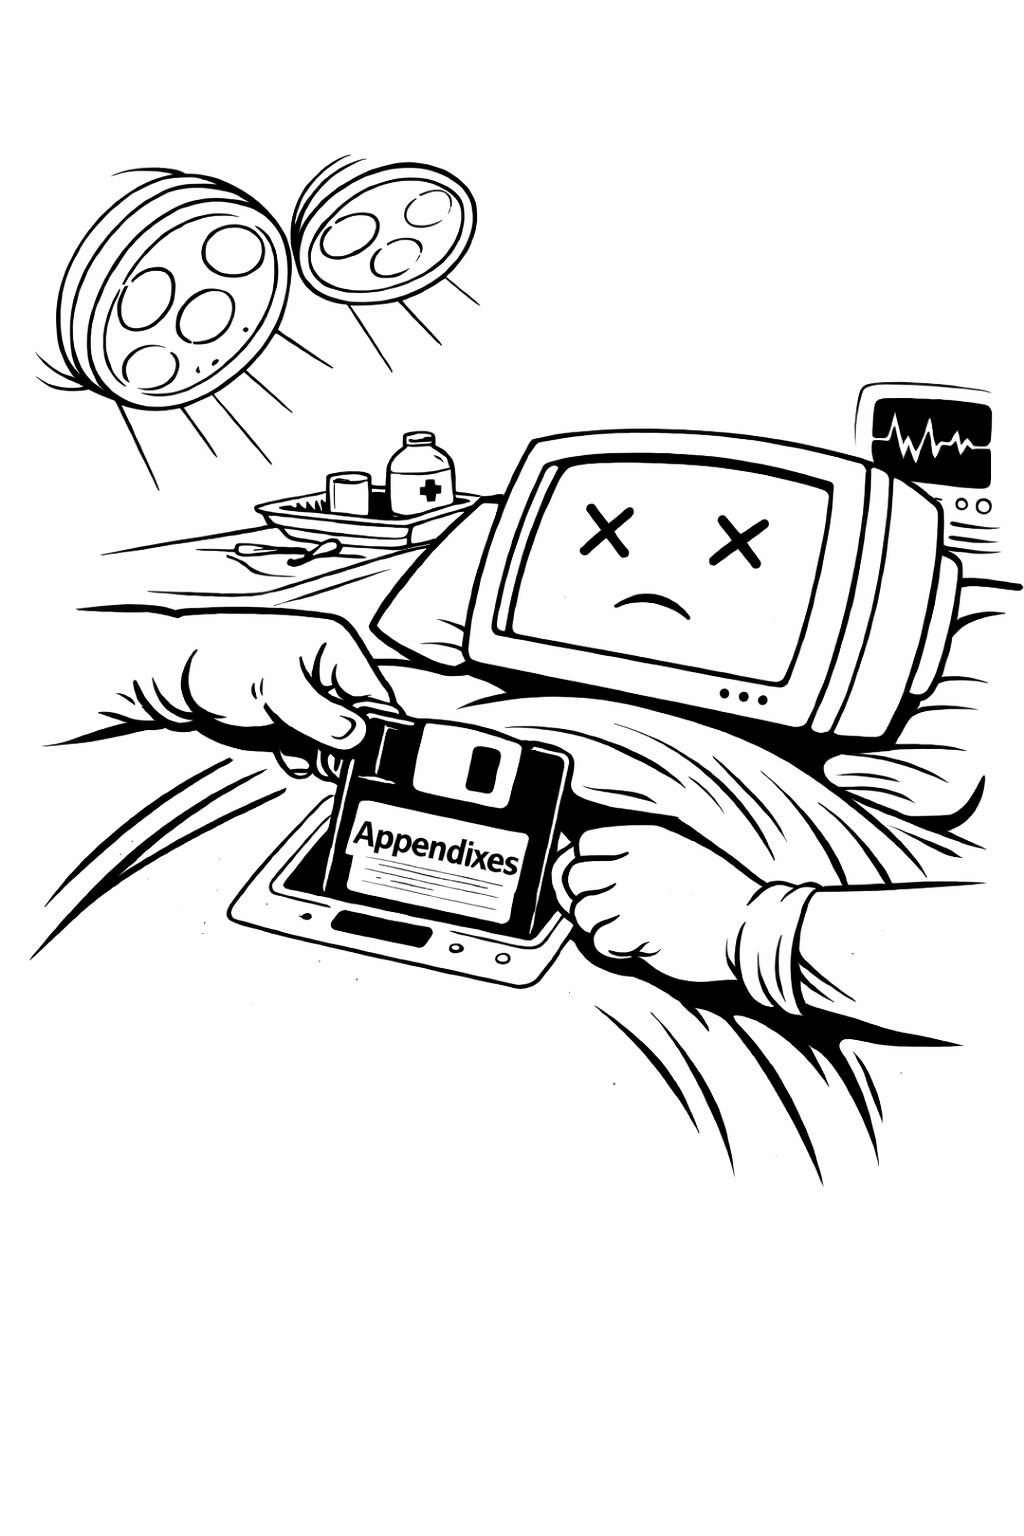
\includegraphics[width=0.85\textwidth]{servidor_app_v2.png}
\end{center}
\vspace*{\fill}

\cleardoublepage
\appendix
% appendices/A_glossary.tex
\chapter{Beginner Glossary}
\label{app:glossary}



This glossary explains common terms used throughout the manual.

\section*{Core concepts}
\addcontentsline{toc}{section}{Core concepts}

\begin{description}[leftmargin=!,labelwidth=4cm]
  \item[Terminal] A text-based interface where you type commands for the operating system.
  \item[Command] A short instruction you type in the terminal (e.g., \texttt{sudo apt update}).
  \item[sudo] ``Run as administrator'' on Linux. Required for system-level changes.
  \item[Package manager (APT)] A tool that installs and updates software on Debian/Ubuntu (\texttt{apt}).
  \item[Repository] A source of software packages that \texttt{apt} can download from.
  \item[GPG key] A cryptographic key used to verify that packages come from the real publisher and were not modified.
\end{description}

\section*{Docker terms}
\addcontentsline{toc}{section}{Docker terms}

\begin{description}[leftmargin=!,labelwidth=4cm]
  \item[Docker] A system to run applications in containers.
  \item[Container] A lightweight isolated environment that runs an application with its dependencies.
  \item[Image] A packaged template used to create containers (like an app ``installer'', but for containers).
  \item[Volume] A folder where containers store persistent data on the host disk.
  \item[Docker Compose] A tool to define and run multi-container setups using a YAML file.
  \item[Port] A network entry point (e.g., \texttt{8080}) used to reach a service from a browser or an app.
\end{description}

\section*{Remote access and security}
\addcontentsline{toc}{section}{Remote access and security}

\begin{description}[leftmargin=!,labelwidth=4cm]
  \item[SSH] Secure remote login to a Linux machine (terminal access over the network).
  \item[Firewall] A system that controls which network traffic is allowed in/out.
  \item[VPN] A private network tunnel that lets you access services securely as if you were on the local network.
\end{description} 
% appendices/B_compose_files.tex
\chapter{Compose Files (copy/paste reference)}
\label{app:compose}

\section{How to use this appendix}
This appendix collects the Docker Compose files used throughout the manual in one place.

\subsection*{A small bit of theory (so the files make sense)}
\begin{itemize}[leftmargin=*]
  \item \textbf{YAML indentation matters.} Use spaces, not tabs.
  \item Lines starting with \texttt{\#} are \textbf{comments} (ignored by Docker).
  \item Many files use a \texttt{.env} file in the same folder to store passwords and variables.
  \item Use this workflow:
\end{itemize}

\begin{lstlisting}
cd /srv/docker/compose/SERVICE
nano .env
nano docker-compose.yml
docker compose up -d
\end{lstlisting}

\encourage{Copy/paste is not cheating. It is how servers are built.}

\section{B.1 PhotoPrism (with MariaDB)}
\subsection*{Folder}
\begin{lstlisting}
/srv/docker/compose/photoprism
\end{lstlisting}

\subsection*{.env}
\begin{lstlisting}
# --- PhotoPrism admin login ---
PHOTOPRISM_ADMIN_USER=admin
PHOTOPRISM_ADMIN_PASSWORD=CHANGE_THIS_TO_A_LONG_PASSWORD

# --- Database (MariaDB) ---
MARIADB_DATABASE=photoprism
MARIADB_USER=photoprism
MARIADB_PASSWORD=CHANGE_THIS_DB_PASSWORD
MARIADB_ROOT_PASSWORD=CHANGE_THIS_ROOT_PASSWORD

# --- Optional: match your Linux user (helps avoid permission issues) ---
PHOTOPRISM_UID=1000
PHOTOPRISM_GID=1000
\end{lstlisting}

\subsection*{docker-compose.yml}
\begin{lstlisting}
services:
  mariadb:
    image: mariadb:11
    container_name: photoprism-mariadb
    restart: unless-stopped
    environment:
      MARIADB_DATABASE: ${MARIADB_DATABASE}
      MARIADB_USER: ${MARIADB_USER}
      MARIADB_PASSWORD: ${MARIADB_PASSWORD}
      MARIADB_ROOT_PASSWORD: ${MARIADB_ROOT_PASSWORD}
    volumes:
      - /srv/photos/mariadb:/var/lib/mysql

  photoprism:
    image: photoprism/photoprism:latest
    container_name: photoprism
    restart: unless-stopped
    depends_on:
      - mariadb
    ports:
      - "2342:2342"
    environment:
      PHOTOPRISM_ADMIN_USER: ${PHOTOPRISM_ADMIN_USER}
      PHOTOPRISM_ADMIN_PASSWORD: ${PHOTOPRISM_ADMIN_PASSWORD}

      PHOTOPRISM_DATABASE_DRIVER: "mysql"
      PHOTOPRISM_DATABASE_SERVER: "mariadb:3306"
      PHOTOPRISM_DATABASE_NAME: ${MARIADB_DATABASE}
      PHOTOPRISM_DATABASE_USER: ${MARIADB_USER}
      PHOTOPRISM_DATABASE_PASSWORD: ${MARIADB_PASSWORD}

      PHOTOPRISM_UID: ${PHOTOPRISM_UID}
      PHOTOPRISM_GID: ${PHOTOPRISM_GID}

      PHOTOPRISM_SITE_URL: "http://localhost:2342/"
      PHOTOPRISM_ORIGINALS_LIMIT: 5000
    volumes:
      - /srv/photos/originals:/photoprism/originals
      - /srv/photos/import:/photoprism/import
      - /srv/photos/storage:/photoprism/storage
\end{lstlisting}

\section{B.2 Navidrome}
\subsection*{Folder}
\begin{lstlisting}
/srv/docker/compose/navidrome
\end{lstlisting}

\subsection*{.env}
\begin{lstlisting}
ND_SCANSCHEDULE=1h
ND_LOGLEVEL=info
TZ=Europe/Madrid
\end{lstlisting}

\subsection*{docker-compose.yml}
\begin{lstlisting}
services:
  navidrome:
    image: deluan/navidrome:latest
    container_name: navidrome
    restart: unless-stopped
    ports:
      - "4533:4533"
    environment:
      ND_SCANSCHEDULE: ${ND_SCANSCHEDULE}
      ND_LOGLEVEL: ${ND_LOGLEVEL}
      TZ: ${TZ}
    volumes:
      - /srv/music/data:/data
      - /srv/music/library:/music:ro
\end{lstlisting}

\section{B.3 Local AI (Ollama + Open WebUI)}
\subsection*{Folder}
\begin{lstlisting}
/srv/docker/compose/local-ai
\end{lstlisting}

\subsection*{docker-compose.yml}
\begin{lstlisting}
services:
  ollama:
    image: ollama/ollama:latest
    container_name: ollama
    ports:
      - "11434:11434"
    environment:
      TZ: Europe/Madrid
    volumes:
      - /srv/ai/ollama:/root/.ollama
    restart: unless-stopped

  open-webui:
    image: ghcr.io/open-webui/open-webui:main
    container_name: open-webui
    ports:
      - "3000:8080"
    environment:
      OLLAMA_BASE_URL: "http://ollama:11434"
      TZ: Europe/Madrid
    volumes:
      - /srv/ai/openwebui:/app/backend/data
    depends_on:
      - ollama
    restart: unless-stopped
\end{lstlisting}

\subsection*{Optional: enable NVIDIA GPU acceleration (snippet)}
If you have an NVIDIA GPU, add the following block \textbf{inside the \texttt{ollama:} service},
at the same indentation level as \texttt{restart}, \texttt{ports}, and \texttt{volumes}.
\textbf{Note:} GPU acceleration requires NVIDIA drivers and NVIDIA Container Toolkit (Linux) or Docker Desktop GPU support (Windows).

\begin{lstlisting}
  ollama:
    image: ollama/ollama:latest
    container_name: ollama
    ports:
      - "11434:11434"
    environment:
      TZ: Europe/Madrid
    volumes:
      - /srv/ai/ollama:/root/.ollama
    restart: unless-stopped
    deploy:
      resources:
        reservations:
          devices:
            - driver: nvidia
              count: all
              capabilities: [gpu]
\end{lstlisting}

Then restart the stack:
\begin{lstlisting}
docker compose down
docker compose up -d
\end{lstlisting}

\subsection*{Verification}
First, verify GPU on the host:
\begin{lstlisting}
nvidia-smi
docker ps
\end{lstlisting}

If available inside the container (not always):
\begin{lstlisting}
docker exec -it ollama nvidia-smi
\end{lstlisting}

If your Compose ignores \texttt{deploy:} on your system, see Chapter 7 (GPU troubleshooting) for the alternative \texttt{--gpus all} approach.

\section{B.4 Nextcloud (core stack)}
\subsection*{Folder}
\begin{lstlisting}
/srv/docker/compose/nextcloud
\end{lstlisting}

\subsection*{.env}
\begin{lstlisting}
MYSQL_DATABASE=nextcloud
MYSQL_USER=nextcloud
MYSQL_PASSWORD=CHANGE_THIS_DB_PASSWORD
MYSQL_ROOT_PASSWORD=CHANGE_THIS_ROOT_PASSWORD

NEXTCLOUD_ADMIN_USER=admin
NEXTCLOUD_ADMIN_PASSWORD=CHANGE_THIS_TO_A_LONG_PASSWORD

# Space-separated:
NEXTCLOUD_TRUSTED_DOMAINS=localhost 127.0.0.1 SERVER_IP

TZ=Europe/Madrid
\end{lstlisting}

\subsection*{docker-compose.yml (core)}
\begin{lstlisting}
services:
  db:
    image: mariadb:11
    container_name: nextcloud-db
    restart: unless-stopped
    command: --transaction-isolation=READ-COMMITTED --binlog-format=ROW
    environment:
      MYSQL_DATABASE: ${MYSQL_DATABASE}
      MYSQL_USER: ${MYSQL_USER}
      MYSQL_PASSWORD: ${MYSQL_PASSWORD}
      MYSQL_ROOT_PASSWORD: ${MYSQL_ROOT_PASSWORD}
      TZ: ${TZ}
    volumes:
      - /srv/drive/nextcloud/db:/var/lib/mysql

  redis:
    image: redis:7-alpine
    container_name: nextcloud-redis
    restart: unless-stopped
    command: redis-server --appendonly yes
    volumes:
      - /srv/drive/nextcloud/redis:/data

  app:
    image: nextcloud:apache
    container_name: nextcloud
    restart: unless-stopped
    depends_on:
      - db
      - redis
    ports:
      - "8080:80"
    environment:
      MYSQL_HOST: db
      MYSQL_DATABASE: ${MYSQL_DATABASE}
      MYSQL_USER: ${MYSQL_USER}
      MYSQL_PASSWORD: ${MYSQL_PASSWORD}
      NEXTCLOUD_ADMIN_USER: ${NEXTCLOUD_ADMIN_USER}
      NEXTCLOUD_ADMIN_PASSWORD: ${NEXTCLOUD_ADMIN_PASSWORD}
      NEXTCLOUD_TRUSTED_DOMAINS: ${NEXTCLOUD_TRUSTED_DOMAINS}
      TZ: ${TZ}
    volumes:
      - /srv/drive/nextcloud/html:/var/www/html
      - /srv/drive/nextcloud/data:/var/www/html/data

  cron:
    image: nextcloud:apache
    container_name: nextcloud-cron
    restart: unless-stopped
    depends_on:
      - app
    entrypoint: /cron.sh
    volumes:
      - /srv/drive/nextcloud/html:/var/www/html
      - /srv/drive/nextcloud/data:/var/www/html/data
\end{lstlisting}

\subsection*{Optional: add OnlyOffice Docs (service snippet)}
Add inside \texttt{services:}:

\begin{lstlisting}
  onlyoffice:
    image: onlyoffice/documentserver:latest
    container_name: onlyoffice
    restart: unless-stopped
    environment:
      TZ: ${TZ}
      JWT_ENABLED: "true"
      JWT_SECRET: "CHANGE_THIS_TO_A_LONG_RANDOM_SECRET"
    ports:
      - "8081:80"
\end{lstlisting}

\section{B.5 Seafile (core stack)}
\subsection*{Folder}
\begin{lstlisting}
/srv/docker/compose/seafile
\end{lstlisting}

\subsection*{.env}
\begin{lstlisting}
SEAFILE_SERVER_HOSTNAME=SERVER_IP

SEAFILE_ADMIN_EMAIL=admin@example.com
SEAFILE_ADMIN_PASSWORD=CHANGE_THIS_TO_A_LONG_PASSWORD

MYSQL_ROOT_PASSWORD=CHANGE_THIS_ROOT_PASSWORD
MYSQL_LOG_CONSOLE=true

TZ=Europe/Madrid
\end{lstlisting}

\subsection*{docker-compose.yml (core)}
\begin{lstlisting}
services:
  db:
    image: mariadb:11
    container_name: seafile-db
    restart: unless-stopped
    environment:
      MYSQL_ROOT_PASSWORD: ${MYSQL_ROOT_PASSWORD}
      MYSQL_LOG_CONSOLE: ${MYSQL_LOG_CONSOLE}
      TZ: ${TZ}
    volumes:
      - /srv/drive/seafile-db:/var/lib/mysql

  memcached:
    image: memcached:1.6-alpine
    container_name: seafile-memcached
    restart: unless-stopped

  seafile:
    image: seafileltd/seafile-mc:latest
    container_name: seafile
    restart: unless-stopped
    depends_on:
      - db
      - memcached
    ports:
      - "8000:80"
    environment:
      DB_HOST: db
      DB_ROOT_PASSWD: ${MYSQL_ROOT_PASSWORD}
      TIME_ZONE: ${TZ}
      SEAFILE_ADMIN_EMAIL: ${SEAFILE_ADMIN_EMAIL}
      SEAFILE_ADMIN_PASSWORD: ${SEAFILE_ADMIN_PASSWORD}
      SEAFILE_SERVER_HOSTNAME: ${SEAFILE_SERVER_HOSTNAME}
    volumes:
      - /srv/drive/seafile:/shared
\end{lstlisting}

\subsection*{Optional: add OnlyOffice Docs (service snippet)}
Add inside \texttt{services:}:

\begin{lstlisting}
  onlyoffice:
    image: onlyoffice/documentserver:latest
    container_name: seafile-onlyoffice
    restart: unless-stopped
    environment:
      TZ: ${TZ}
      JWT_ENABLED: "true"
      JWT_SECRET: "CHANGE_THIS_TO_A_LONG_RANDOM_SECRET"
    ports:
      - "8001:80"
\end{lstlisting}




\section{B.6 Notes on placeholders}
Replace these placeholders before running:
\begin{itemize}[leftmargin=*]
  \item \texttt{SERVER\_IP} with your server IP (see Chapter~\ref{ch:theory_compose_yaml}),
  \item passwords marked \texttt{CHANGE\_THIS\_*} with strong passwords,
  \item emails like \texttt{admin@example.com} with your real admin email.
\end{itemize}

\encourage{If you keep your Compose files and \texttt{/srv} backups, you can rebuild the entire system. That is the quiet superpower of this manual.} 
% appendices/C_vpn_remote_access.tex
\chapter{Optional: Remote access with VPN (recommended)}
\label{app:vpn}

\section{Goal}
This appendix explains how to access your self-hosted services (PhotoPrism, Navidrome, etc.)
from outside your home network \emph{without} exposing them publicly to the internet.

By the end, you will:
\begin{itemize}[leftmargin=*]
  \item understand why VPN is the safest beginner-friendly approach,
  \item choose a VPN method that fits your environment,
  \item verify remote access using the same local URLs (e.g., \texttt{http://SERVER\_IP:2342}).
\end{itemize}

\encourage{Remote access is where many projects go off the rails. A VPN keeps it simple: instead of making your services public, you make \emph{your device private}.}

\section{The key idea (one sentence)}
A VPN makes your phone/laptop behave as if it were on your home Wi-Fi, even when you are away.

That means: if PhotoPrism works at home with
\begin{lstlisting}
http://SERVER_IP:2342
\end{lstlisting}
it should work the same way over VPN.

\section{Before you start: avoid the ``open ports'' trap}
A common beginner instinct is: ``I will just open a port on my router.''
This can work, but it often leads to:
\begin{itemize}[leftmargin=*]
  \item security mistakes (public exposure without TLS),
  \item router/ISP limitations (CGNAT),
  \item complicated reverse-proxy setups.
\end{itemize}

VPN is usually the safer, shorter path.

\section{Choose your VPN approach}
There is no single perfect solution for everyone. Pick the one that matches your situation.

\subsection{Option 1: Use an existing VPN (simplest if you already have one)}
Some people already have a VPN provided by their workplace or university.

\textbf{How it works:}
\begin{itemize}[leftmargin=*]
  \item Connect your phone/laptop to that VPN.
  \item If your server is reachable through the VPN network, you can access services using the server IP.
\end{itemize}

\textbf{When this is enough:}
\begin{itemize}[leftmargin=*]
  \item your server is inside that VPN network (or reachable through it),
  \item you only need access for yourself (not for many external users).
\end{itemize}

\encourage{If you already have a VPN that reaches your server: congrats, you may already be done.}


\subsection{Option 2: Tailscale (step-by-step, least friction)}
Tailscale is a mesh VPN built on WireGuard. Many people like it because it works even when:
\begin{itemize}[leftmargin=*]
  \item you cannot easily configure your router,
  \item your ISP uses CGNAT,
  \item you want device-to-device access with minimal networking work.
\end{itemize}

\encourage{This is the ``I just want it to work'' option. Follow the steps in order. If something fails, it is almost always because one device is not logged in, or you are not actually connected.}

\subsubsection*{Step 1 --- Create a Tailscale account}
On any computer/phone browser:
\begin{itemize}[leftmargin=*]
  \item Go to the Tailscale website and create an account (for example using Google, Microsoft, GitHub, etc.).
\end{itemize}
You will manage your devices from the Tailscale admin console.

\subsubsection*{Step 2 --- Install Tailscale on the server}
Install it on the machine that runs your services (the same machine that runs Docker).

\paragraph{Linux (Path A).}
Install using the official Tailscale script (simple and common):
\begin{lstlisting}
curl -fsSL https://tailscale.com/install.sh | sh
\end{lstlisting}

Then bring the server online:
\begin{lstlisting}
sudo tailscale up
\end{lstlisting}

\textbf{What happens now:}
\begin{itemize}[leftmargin=*]
  \item A browser window (or a URL in the terminal) will ask you to log in.
  \item After login, the server becomes a device in your Tailscale network.
\end{itemize}

\paragraph{Windows (Path B).}
Install the Tailscale application on Windows (standard installer).
Then sign in with the same account.
(You can run Tailscale on Windows even if your Docker workflow uses WSL2.)

\subsubsection*{Step 3 --- Install Tailscale on your phone/tablet/laptop}
Install Tailscale on the device you want to use remotely:
\begin{itemize}[leftmargin=*]
  \item phone/tablet: install the Tailscale app from your app store,
  \item laptop: install the Tailscale client for your OS.
\end{itemize}
Log in with the same Tailscale account.

\subsubsection*{Step 4 --- Find your server's Tailscale IP}
Each device gets a stable private IP (often in the \texttt{100.x.y.z} range).

On the server, run:
\begin{lstlisting}
tailscale ip -4
\end{lstlisting}

Or check the device in the Tailscale admin console (it shows the IP and device name).


\encourage{When using Tailscale, you typically use the Tailscale IP (often \texttt{100.x.y.z}), not your home Wi-Fi IP (often \texttt{192.168.x.x}).}

\subsubsection*{Step 5 --- Access services using the Tailscale IP}
Once your phone/laptop is connected to Tailscale, open:

\begin{lstlisting}
http://TAILSCALE_IP:2342   % PhotoPrism
http://TAILSCALE_IP:4533   % Navidrome
\end{lstlisting}

\textbf{Important:} This works from outside your home because your device is now inside your private VPN.

\encourage{If you can load PhotoPrism over mobile data while connected to Tailscale: you have achieved remote access without exposing anything publicly. That is a big win.}

\subsubsection*{Verification checklist (Tailscale)}
You are done when:
\begin{itemize}[leftmargin=*]
  \item the server appears as ``connected'' in Tailscale,
  \item your phone/laptop is connected in the Tailscale app,
  \item you can access \texttt{http://TAILSCALE\_IP:2342} from outside your home Wi-Fi.
\end{itemize}

\subsubsection*{Common pitfalls (Tailscale)}
\begin{itemize}[leftmargin=*]
  \item \textbf{You are still on Wi-Fi and think it works ``remotely''.}
  Test properly: disable Wi-Fi (use mobile data), connect Tailscale, then try again.
  \item \textbf{Wrong IP.} Use the Tailscale IP (often \texttt{100.x.y.z}), not your home LAN IP (e.g., \texttt{192.168.x.x}).
  \item \textbf{Not actually connected.} Open the Tailscale app and confirm ``Connected''.
  \item \textbf{Firewall blocks.} Rare, but if needed, allow inbound connections on the server for local ports (2342, 4533) on the Tailscale interface.
\end{itemize}

\subsection{Option 3 (advanced): WireGuard (classic self-hosted VPN)}
WireGuard is a modern VPN protocol known for simplicity and performance.

\textbf{High-level architecture:}
\begin{itemize}[leftmargin=*]
  \item your server runs a WireGuard VPN endpoint,
  \item your phone/laptop is a WireGuard client,
  \item once connected, your device reaches the server via a private VPN subnet.
\end{itemize}

\textbf{Why it is ``advanced'' here:}
\begin{itemize}[leftmargin=*]
  \item you may need router configuration (port forwarding),
  \item ISP limitations (CGNAT) can complicate inbound connectivity,
  \item you will manage keys and a config file manually.
\end{itemize}

\encourage{WireGuard is worth it if you want maximum control and minimal external dependencies. For this manual, Tailscale remains the recommended default because it has the least friction for beginners.}


\section{Verification checklist (for any VPN option)}
You have remote access when:
\begin{itemize}[leftmargin=*]
  \item your device shows ``VPN connected'',
  \item you can reach the server IP (or VPN IP) from your device,
  \item PhotoPrism/Navidrome load from outside your home network.
\end{itemize}

A practical test:
\begin{itemize}[leftmargin=*]
  \item turn off Wi-Fi on your phone (use mobile data),
  \item connect the VPN,
  \item open \texttt{http://SERVER\_IP:2342} (or VPN IP).
\end{itemize}

\section{Common pitfalls}
\subsection*{It works at home but not outside}
Most likely: you are not actually reaching your home network.
Check that your VPN is connected \emph{and} that it routes traffic to your home subnet.

\subsection*{CGNAT or ISP restrictions}
Some ISPs prevent inbound connections to your home. This makes classic port-forwarding VPN setups harder.
In these cases, solutions like Tailscale often work more smoothly.

\subsection*{Firewall blocking}
If the VPN connects but services do not load, check:
\begin{itemize}[leftmargin=*]
  \item server firewall rules,
  \item Windows firewall (if applicable),
  \item whether the service is bound to the correct interface (usually OK with Docker port publishing).
\end{itemize}

\subsection*{Security reminder}
VPN access still deserves strong passwords and updates.
A VPN is not a substitute for basic hygiene; it is a safer network boundary.

\section{Where to go next}
If you want an even more independent setup, the next upgrade is a full \textbf{WireGuard quickstart}
(self-hosted and fully under your control). For most users, Tailscale is already an excellent solution. 
% appendices/appendix_terminator.tex
\cleardoublepage
\thispagestyle{empty}

\vspace*{\fill}
\begin{center}
  
\includegraphics[width=0.85\textwidth]{servidor_goku.png}
\end{center}
\vspace*{\fill}

\cleardoublepage 
% \input{appendices/B_troubleshooting}
% \input{appendices/C_backups_security}

\end{document} 